% !TeX spellcheck = en_US
\documentclass[review,10pt]{JMtemplate}
\usepackage{bm}
\usepackage{times}
\usepackage{graphicx}
\usepackage{paralist,algorithmic,algorithm}
\usepackage{amsmath,mathrsfs,amssymb}
\usepackage{amsfonts}       % blackboard math symbols
\usepackage{nicefrac}       % compact symbols for 1/2, etc.
\usepackage{microtype}      % microtypography
\usepackage{booktabs}       % professional-quality tables
\usepackage{longtable}
\usepackage{threeparttable}
\usepackage{multirow}
\usepackage{multicol}
\usepackage{soul}
\usepackage{subfigure}
\usepackage{wrapfig}
\usepackage[american]{babel}
\usepackage{algorithm}
\usepackage{algorithmic}
\usepackage{setspace}
\usepackage{stfloats}
\usepackage{lipsum}
\usepackage{multicol}
\usepackage{url}
%\usepackage{siunitx}   % 用于书写 数字+单位 的格式
%\usepackage{upgreek}   % 用于书写 数字+单位 的格式
%\usepackage{xcolor}    % colors
%\usepackage{helvet}
%\usepackage{courier}
\usepackage{makecell}   % 多行换行
\usepackage{hyperref}

\usepackage{natbib}  % DO NOT CHANGE THIS AND DO NOT ADD ANY OPTIONS TO IT
\usepackage{caption} % DO NOT CHANGE THIS AND DO NOT ADD ANY OPTIONS TO IT

\newcommand*{\dif}{\mathop{}\!\mathrm{d}}
\newcommand*{\tr}{\mathop{}\!\mathrm{tr}}
\newcommand*{\diag}{\mathop{}\!\mathrm{diag}}
\newcommand*{\re}{\mathop{}\!\mathrm{Re}}
\newcommand*{\im}{\mathop{}\!\mathrm{Im}}
\newcommand*{\e}{\mathop{}\!\mathrm{e}}
\newcommand*{\ii}{\mathop{}\!\mathrm{i}}
\newcommand*{\op}{\mathop{}\!\mathrm{o}_{\mathrm{P}}}

\newtheorem{theorem}{Theorem}
%\newtheorem{lemma}{Lemma}
\newtheorem{definition}{Definition}
\newtheorem{corollary}[theorem]{Corollary}
\newtheorem{proposition}{Proposition}
\newtheorem{assumption}{Assumption}
\newenvironment{proof}{{\noindent\it Proof.}\quad}{\hfill $\square$\par}


% \include{Manual/Sec_Notations}
% \clearpage
% \include{Manual/Sec_Spiking}


\begin{document}
\begin{frontmatter}
\title{A Unified Kernel for Neural Network Learning}

\author{Shao-Qun Zhang\textsuperscript{a,b,}\footnote{Shao-Qun Zhang is the corresponding author. Email: zhangsq@lamda.nju.edu.cn. Other authors made equal contributions.}}
\author{Zong-Yi Chen\textsuperscript{b}}
\author{Yong-Ming Tian\textsuperscript{b}}
\author{Xun Lu\textsuperscript{b}}
\address{
\textsuperscript{a} National Key Laboratory for Novel Software Technology, Nanjing University, Nanjing 210023, China \\
\textsuperscript{b} School of Intelligent Science and Technology, Nanjing University, Suzhou 215163, China
}
\date{\today}


\begin{abstract}
Past decades have witnessed a great interest in the distinction and connection between neural network learning and kernel learning. Recent advancements have made theoretical progress in connecting infinite-wide neural networks and Gaussian processes. Two predominant approaches have emerged: the Neural Network Gaussian Process (NNGP) and the Neural Tangent Kernel (NTK). The former, rooted in Bayesian inference, represents a zero-order kernel, while the latter, grounded in the tangent space of gradient descents, is a first-order kernel. In this paper, we present the Unified Neural Kernel (UNK), which characterizes the learning dynamics of neural networks with gradient descents and parameter initialization. The proposed UNK kernel maintains the limiting properties of both NNGP and NTK, exhibiting behaviors akin to NTK with a finite learning step and converging to NNGP as the learning step approaches infinity. Besides, we also theoretically characterize the uniform tightness and learning convergence of the UNK kernel, providing comprehensive insights into this unified kernel. Experimental results underscore the effectiveness of our proposed method. \vspace{0.5cm}
\end{abstract}


\begin{keyword}
Neural Network Learning \sep
Unified Neural Kernel \sep
Neural Network Gaussian Process \sep
Neural Tangent Kernel \sep
Gradient Descent \sep
Uniform Tightness \sep
Convergence \sep
Optimal Trajectory
\end{keyword}


\end{frontmatter}


% This equivalence facilitates precise approximations of the behavior of infinite-wide Bayesian neural networks without resorting to variational inference. Relatively, it also allows for the characterization of the distribution of randomly initialized neural networks optimized by gradient descent, eliminating the need to actually run an optimizer for such analyses. 

\section{Introduction}  \label{sec:introduction}
While neural network learning is successful in a number of applications, it is not yet well understood theoretically \citep{poggio2020theoretical}. Recently, there has been an increasing amount of literature exploring the correspondence between infinite-wide neural networks and Gaussian processes~\citep{neal1996:GP}. Researchers have identified equivalence between the two in various architectures~\citep{garriga2019:GP,novak2018:GP,yang2019:GP}. This equivalence facilitates precise approximations of the behavior of infinite-wide Bayesian neural networks without resorting to variational inference. Relatively, it also allows for the characterization of the distribution of randomly initialized neural networks optimized by gradient descent, eliminating the need to actually run an optimizer for such analyses. 


The standard investigation in this field encompasses the Neural Network Gaussian Process (NNGP)~\citep{lee2018:NNGP}, which establishes that a neural network converges to a Gaussian process statistically as its width approaches infinity. The NNGP kernel inherently induces a posterior distribution that aligns with the feed-forward inference of infinite-wide Bayesian neural networks employing an i.i.d. Gaussian prior. Another typical work is the Neural Tangent Kernel (NTK)~\citep{jacot2018:NTK}, where the function of a neural network trained through gradient descent converges to the kernel gradient of the functional cost as the width of the neural network tends to infinity. The NTK kernel captures the learning dynamic wherein learned parameters are closely tied to their initialization, resembling an i.i.d. Gaussian prior. These two kernels, derived from neural networks, exhibit distinct characteristics based on different initializations and regularization. A notable contrast lies in the fact that the NNGP, rooted in Bayesian inference, represents a zero-order kernel that are more suitable to describe the overall characteristics of neural network learning. In contrast, the NTK, rooted in the tangent space of gradient descents, is a first-order kernel that is adept at capturing local characteristics of neural network learning. Empirical evidence provided by Lee et al.~\citep{lee2020finite} demonstrates the divergent generalization performances of these two kernels across various datasets.



In this paper, we undertake an endeavor to unify both the NNGP and NTK kernels and present the Unified Neural Kernel (UNK) as a cohesive framework for neural network learning. By leveraging the learning dynamics associated with gradient descents and parameter initialization, we delve into theoretical characterizations, including but not limited to the existence, limiting properties, uniform tightness, and learning convergence of the proposed UNK kernel. Our theoretical investigations reveal that the UNK kernel exhibits behaviors reminiscent of the NTK kernel with a finite learning step and converges to the NNGP kernel as the learning step approaches infinity. This contribution not only significantly expands the scope of the existing elegant theory connecting kernel learning and neural network learning, but also represents a substantial step toward unraveling the true intricacies of deep learning.

Our main contributions can be summarized as follows:
\begin{itemize}
    \item We propose the UNK kernel, built upon the learning dynamics associated with gradient descents and parameter initialization, which unifies the limiting properties of both the NTK and NNGP kernels.
    \item We theoretically investigate the asymptotic behaviors of the proposed UNK kernel, in which the UNK kernel is uniformly tight on the space of continuous functions and maintains a tight bound for the smallest eigenvalue.
    \item We conduct experiments on benchmark datasets using various configurations. The numerical results further underscore the effectiveness of our proposed method.
\end{itemize}

The rest of this paper is organized as follows. Section~\ref{sec:pre} introduces useful notations, terminologies, and related studies. Section~\ref{sec:unify} presents the UNK kernel with in-depth discussions and proof sketches. Section~\ref{sec:properties} shows the uniform tightness and convergence of the UNK kernel. Section~\ref{sec:experiments} conducts numerical experiments. Section~\ref{sec:conclusions} concludes our work.


\section{Preliminary}  \label{sec:pre}
This section will introduce useful notations, terminologies, and related studies.

\subsection{Notations}  \label{subsec:notations}
Let $[N] = \{1, 2, \dots, N\}$ be an integer set for $N \in \mathbb{N}^+$, and $|\cdot|_{\#}$ denotes the number of elements in a collection, e.g., $|[N]|_{\#} = N$. Given two functions $g,h\colon \mathbb{N}^+\rightarrow \mathbb{R}$, we denote by $h=\mathbf{\Theta}(g)$ if there exist positive constants $c_1,c_2$, and $n_0$ such that $c_1g(n) \leq h(n) \leq c_2g(n)$ for every $n \geq n_0$; $h=\mathcal{O}(g)$ if there exist positive constants $c$ and $n_0$ such that $h(n) \leq cg(n)$ for every $n \geq n_0$; $h=\Omega(g)$ if there exist positive constants $c$ and $n_0$ such that $h(n) \geq cg(n)$ for every $n \geq n_0$. We define the globe $\mathcal{B}(r) = \{ \boldsymbol{x} \mid \| \boldsymbol{x} \|_2 \leq r \}$ for any $r\in\mathbb{R}^+$. Let $\mathbf{I}_n$ be the $n \times n$-dimensional identity matrix. Let $\|\cdot\|_p$ be the norm of a vector or matrix, in which we employ $p=2$ as the default. Given $\boldsymbol{x}=(x_1,\dots,x_n)$ and $\boldsymbol{y}=(y_1,\dots,y_n)$, we also define the sup-related measure as $\| \boldsymbol{x} - \boldsymbol{y} \|_{\alpha}^{\textrm{sup}} = \sup_{i\in[n]} \big| x_i - y_i \big|^{\alpha}$ for $\alpha>0$.



Let $\mathcal{C}(\mathbb{R}^{n_0};\mathbb{R}^n)$ be the space of continuous functions where $n_0,n\in\mathbb{N}$. Provided a linear and bounded functional $\mathcal{F}: \mathcal{C}(\mathbb{R}^{n_0};\mathbb{R}^n) \to \mathbb{R}$ and a function $f \in  \mathcal{C}(\mathbb{R}^{n_0};\mathbb{R}^n)$ which satisfies $f(\boldsymbol{x}) \overset{\underset{\mathrm{d}}{}}{\to} f^*$, then we have $\mathcal{F} (f(\boldsymbol{x})) \overset{\underset{\mathrm{d}}{}}{\to} \mathcal{F}(f^*)$ and $\mathbb{E} \left[ \mathcal{F} (f(\boldsymbol{x})) \right] \to \mathbb{E} \left[ \mathcal{F}(f^*) \right]$ according to General Transformation Theorem~\citep[Theorem 2.3]{van2000asymptotic} and Uniform Integrability~\citep{billingsley2013convergence}, respectively.

Throughout this paper, we use the specific symbol $K$ to denote the concerned kernel for neural network learning. The superscript $(l)$ and stamp $t$ are used for recording the indexes of hidden layers and training epochs, respectively. We denote the Gaussian distribution by $\mathcal{N}(\mu_x, \sigma_x^2)$, where $\mu_x$ and $\sigma_x^2$ indicate the mean and variance, respectively. In general, we employ $\mathbb{E}(\cdot)$ and $\mathrm{Var}(\cdot)$ to denote the expectation and variance, respectively.




\subsection{NNGP and NTK}  \label{subsec:two_kernels}
We start this work with an $L$-hidden-layer fully-connected neural networks, where $n_l$ and $n_0$ indicate the number of neurons in the $l$-th hidden layer for $l \in [L]$ and input, respectively, as follows
\begin{equation} \label{eq:feedforward}
	\left\{~\begin{aligned}
		\boldsymbol{s}^{(0)} &= \boldsymbol{x} \ , \\
		\boldsymbol{h}^{(l)} &= \mathbf{W}^{(l)} \boldsymbol{s}^{(l-1)} + \boldsymbol{b}^{(l)} \ ,\quad l \in [L] \ , \\
		\boldsymbol{s}^{(l)} &= \phi( \boldsymbol{h}^{(l)} ) \ ,\quad l \in [L] \ , \\
		\boldsymbol{y} &= \boldsymbol{s}^{L} \ ,
	\end{aligned}\right.
\end{equation}
in which $\boldsymbol{x} \in \mathbb{R}^{n_0}$ and $\boldsymbol{y} \in \mathbb{R}^{n_L}$ indicate the variables of inputs respectively, $\boldsymbol{h}^{(l)} \in \mathbb{R}^{n_l}$ and $\boldsymbol{s}^{(l)} \in \mathbb{R}^{n_l}$ denote the pre-synaptic and post-synaptic variables of the $l$-th hidden layer respectively,  $\mathbf{W}^{(l)} \in \mathbb{R}^{n_l \times n_{l-1}} $ and $\boldsymbol{b}^{(l)} \in \mathbb{R}^{n_l} $ are the parameter variables of connection weights and bias respectively, and $\phi$ is an element-wise activation function. For convenience, we here note the parameter variables at the $t$-th epoch as $\Theta^{(l)}_t = [ \mathbf{W}^{(l)}, \boldsymbol{b}^{(l)} ]$, and $\Theta^{(l)}_0$ denotes the initialized parameters, of which the value obeys the Gaussian distribution $\mathcal{N}(0, \sigma^2/n_l)$.


\vspace{0.2 cm}
\noindent\textbf{Neural Network Gaussian Process (NNGP).} For any $l \in [L]$, there is a claim that the conditional variable $\boldsymbol{h}^{(l)} \mid 	\boldsymbol{s}^{(l-1)}$ obeys the Gaussian distribution. In detail, one has $\textrm{Var} ( \boldsymbol{h}^{(l)} \mid	\boldsymbol{s}^{(l-1)} ) = \textrm{Var} ( \mathbf{W}^{(l)}) \mathbb{E} ( \boldsymbol{s}^{(l-1)} )^2 + \textrm{Var} (  \boldsymbol{b}^{(l)} )$, where $\cdot^2$ and $\cdot$ denote the dot product and this equality holds according to $\mathbb{E} ( \mathbf{W}^{(l)} ) = \mathbf{0}$, $\mathbb{E}( \boldsymbol{b}^{(l)} ) = \boldsymbol{0} $, and the mutual independence of elements $\mathbf{W}^{(l)}$ and $\boldsymbol{b}^{(l)}$. It is reasonable to conjecture that $\boldsymbol{s}^{(l-1)} \sim \mathcal{N}(\boldsymbol{0}, \mathbf{I}_{n_{l-1}} / C_{\phi})$ according to the principle of mathematical induction and $\boldsymbol{x} \sim \mathcal{N}(\boldsymbol{0}, \mathbf{I}_{n_0})$, where $C_{\phi} = {1}/{\mathbb{E}_{z \sim \mathcal{N}(0,1)} \left( \phi(z) \right)^2 }$. Hence, one has
\[
\boldsymbol{h}^{(l)} \mid	\boldsymbol{s}^{(l-1)}  \sim \mathcal{N} \left(  \boldsymbol{0}, \frac{\sigma^2}{n_{l-1}} \left( \frac{1}{C_{\phi}} + 1 \right) \mathbf{I}_{n_l} \right) \ .
\]
Moreover, the NNGP kernel is defined by
\[
K_{\textrm{NNGP}}^{(l)} \left( \boldsymbol{s}^{(l-1)}, \boldsymbol{s}'^{(l-1)} \right) 	= \sigma^2 ~\mathbb{E} \left\langle\boldsymbol{s}^{(l-1)},  \boldsymbol{s}'^{(l-1)}  \right\rangle + \sigma^2
\]
with
\[
\lim\limits_{n_{l-1} \to \infty} \mathbb{E} \left\langle \boldsymbol{h}^{(l)} \mid	\boldsymbol{s}^{(l-1)}, \boldsymbol{h}^{(l)} \mid \boldsymbol{s}^{(l-1)}  \right\rangle =  \sigma^2 \left( \frac{1}{C_{\phi}} + 1 \right) \ .
\]



\vspace{0.2 cm}
\noindent\textbf{Neural Tangent Kernel (NTK).} The training of the concerned ANNs consists in optimizing $\boldsymbol{y} = f(\boldsymbol{x} ; \Theta)$ in the function space, supervised by a functional loss $\hbar(\Theta)$, such as the square or cross-entropy functions, where we employ $\Theta$ to denote the variable of any parameter
\[
\frac{\dif \Theta}{\dif t} = - \frac{\dif \hbar(\Theta)}{\dif \Theta} = - \frac{\dif \hbar(\Theta)}{\dif f(\boldsymbol{x} ; \Theta)} \frac{\dif f(\boldsymbol{x} ; \Theta)}{\dif \Theta} \ .
\]
For any $l \geq 2$, there is a claim that the gradient variable vector $\boldsymbol{h}^{(l)} \mid \boldsymbol{s}^{(l-1)}$ obeys the Gaussian distribution. Taking $\mathbf{W}^{(l-1)}$ as an example, one has $\textrm{Var} ( {\partial \boldsymbol{h}^{(l)}}/{\partial \mathbf{W}_{ij}^{(l-1)}} ) = \textrm{Var} ( \mathbf{W}^{(l)} ) \mathbb{E} ( {\partial \boldsymbol{s}^{(l-1)}}/{\partial \boldsymbol{h}^{(l-1)}} )^2 \textrm{Var} (  \boldsymbol{s}^{(l-2)} )$ for $i,j \in \mathbb{N}^+$, where ${\partial \boldsymbol{s}^{(l-1)}} / {\partial \boldsymbol{h}^{(l-1)}}$ adopts the dot operation. Hence, one has
\[
\frac{\partial \boldsymbol{h}^{(l)}}{\partial \mathbf{W}_{ij}^{(l-1)}} \sim \mathcal{N} \left(  \boldsymbol{0}, \frac{\sigma^2}{n_{l-1} C'_{\phi} C_{\phi} } \mathbf{I}_{n_{l-1}} \right)  \ ,
\]
where $C'_{\phi} = {1}/{\mathbb{E}_{z \sim \mathcal{N}(0,1)} \left( \phi'(z) \right)^2 } $. Moreover, the NTK kernel is defined by
\[
\left\{ \begin{aligned}
K_{\textrm{NTK}}^{(1)} \left(  \boldsymbol{x}, \boldsymbol{x}' \right)  &= K_{\textrm{NNGP}}^{(1)} \left(  \boldsymbol{x}, \boldsymbol{x}' \right)  \ , \quad\text{for}\quad l = 1 \ ,  \\
K_{\textrm{NTK}}^{(l)} \left(  \boldsymbol{s}^{(l-1)}, \boldsymbol{s}'^{(l-1)} \right)  &= K_{\textrm{NTK}}^{(l-1)} \left(  \boldsymbol{s}^{(l-2)}, \boldsymbol{s}'^{(l-2)} \right) \mathbb{E} \left\langle \frac{\partial \boldsymbol{s}^{(l-1)}}{\partial \boldsymbol{h}^{(l-1)}},  \frac{\partial \boldsymbol{s}'^{(l-1)}}{\partial \boldsymbol{h}'^{(l-1)}} \right\rangle \\
&\quad + K_{\textrm{NNGP}}^{(l)} \left( \boldsymbol{s}^{(l-1)}, \boldsymbol{s}'^{(l-1)} \right) \ ,
\quad\text{for}\quad l \geq 2 \ , 
\end{aligned} \right.
\]
with
\[
\left\{\begin{aligned}
& \lim\limits_{n_{l-1} \to \infty} \mathbb{E} \left\langle \frac{\partial \boldsymbol{h}^{(l)}}{\partial \mathbf{W}_{ij}^{(l-1)}} , \frac{\partial \boldsymbol{h}^{(l)}}{\partial \mathbf{W}_{ij}^{(l-1)}}  \right\rangle  =  \frac{\sigma^2}{C'_{\phi} C_{\phi} } \ , \\
& \lim\limits_{n_{l-1} \to \infty} \mathbb{E} \left\langle \frac{\partial \boldsymbol{h}^{(l)}}{\partial \boldsymbol{b}_i^{(l-1)} } , \frac{\partial \boldsymbol{h}^{(l)}}{\partial \boldsymbol{b}_i^{(l-1)} }  \right\rangle  =  \frac{\sigma^2}{C'_{\phi} } \ .
\end{aligned} \right.
\]




\subsection{Related Studies}  \label{subsec:rw}
Past decades have witnessed a growing interest in the correspondence between neural network learning and Gaussian processes. Neal et al.~\citep{neal1996:GP} presented the seminal work by showing that a one-hidden-layer network of infinite width turns into a Gaussian process. Cho et al.~\citep{cho2009:GP} linked the multi-layer networks using rectified polynomial activation with compositional Gaussian kernels. Lee et al.~\citep{lee2018:NNGP} showed that the infinitely wide fully connected neural networks with common-used activation functions can converge to Gaussian processes. Recently, the NNGP has been scaled to many types of networks, including Bayesian networks~\citep{novak2018:GP}, deep networks with convolution~\citep{garriga2019:GP}, and recurrent networks~\citep{yang2019:GP}. 

NNGPs can provide a quantitative characterization of how likely certain outcomes are if some aspects of the system are not exactly known. In the experiments of \citep{lee2018:NNGP}, an explicit estimate in the form of variance prediction is given to each test sample. Besides, Pang et al.~\citep{pang2019:NNGP} showed that the NNGP is good at handling data with noise and is superior to discretizing differential operators in solving some linear or nonlinear partial differential equations. Park et al.~\citep{park2020:NNGP} employed the NNGP kernel in the performance measurement of network architectures for the purpose of speeding up the neural architecture search. Pleiss et al.~\citep{pleiss2022:NNGP} leveraged the effects of width on the capacity of neural networks by decoupling the generalization and width of the corresponding NNGP. Despite great progress, numerous studies about NNGP still rely on increasing width to induce the Gaussian processes. Recently, Zhang et al.~\citep{zhang2022:NNGP} proposed a depth paradigm that achieves an NNGP by increasing depth, providing complementary support for the existing theory of NNGP.  

The NTK kernel, first proposed by Jacot et al.~\citep{jacot2018:NTK}, relates a neural network trained by randomly initialized gradient descent with a Gaussian distribution. It has been proved that many types of networks, including graph neural networks on bioinformatics datasets~\citep{du2019:GNTK} and convolution neural network~\citep{arora2019:NTK} on medium-scale datasets like UCI database, can derive a corresponding kernel function. Some researchers applied NTK to various fields, such as federated learning~\citep{huang2021:NTK}, mean-field analysis~\citep{mahankali2023:NTK}, and natural language processing~\citep{malladi2023:NTK}. Recently, Hron et al.~\citep{hron2020:attention} derived the NNGP and NTK from neural networks to multi-head attention architectures as the number of heads tends to infinity. Avidan et al.~\citep{avidan2023:connecting} provided a unified theoretical framework that connects NTK and NNGP using the Markov proximal learning model.



\section{The Unified Kernel} \label{sec:unify}
This work considers a general form of supervised learning 
\begin{equation}  \label{eq:min}
    \min_{\Theta}\quad \hbar(\Theta) + \lambda \mathcal{R}( \Theta )
\end{equation}
where $\mathcal{R}( \Theta )$ is a regularizer and $\lambda$ is the corresponding multiplier. Based on gradient descent, Eq.~\eqref{eq:min} generally leads to a dynamical system with respect to parameter $\Theta$
\begin{equation}  \label{eq:dynamic}
\frac{\dif \Theta}{\dif t} =  -  \frac{\dif \hbar(\Theta)}{\dif \Theta} - \lambda \frac{\dif \mathcal{R}( \Theta ) }{\dif \Theta} \ ,
\end{equation}
where we omit the learning rate for simplicity. From Eq.~\eqref{eq:dynamic}, the value of $\lambda$ can be regarded as a balance between the gradient and regularizer. In the next subsections, we will employ the initialized and epoch-related parameter to implement ${\dif \mathcal{R}( \Theta ) }/{\dif \Theta}$, where both regularization implementations induce the UNK kernel. Furthermore, Subsection~\ref{subsec:experiment_lamda} provides in-depth discussions about the effect of $\lambda$ on the performance of the UNK kernel.


\subsection{Initialization Parameter $\Theta_0$} \label{subsec:initialization}
In this work, we first consider leveraging the effects of initialized parameters\footnote{For example, one just employs the square regularizer in Eq.~\eqref{eq:dynamic}.}, and thus Eq.~\eqref{eq:dynamic} becomes
\begin{equation}  \label{eq:lamda}
\frac{\dif \Theta}{\dif t} =  -  \frac{\dif \hbar(\Theta)}{\dif \Theta} \Big|_t - \lambda \Theta_0 \ ,
\end{equation}
where $\Theta_0$ is the initialized parameter and $\lambda \in \mathbb{R}$ takes a tradeoff between parameter gradient and initialization. 

Now, we present our main conclusion as follows.
\begin{theorem}  \label{thm:unified}
For a network of depth $L$ with a Lipschitz activation $\phi$ and in the limit of the layer width $n_1, \dots, n_{L-1} \to \infty$, Eq.~\eqref{eq:lamda} induces a kernel with the following form, for $l\in[L]$ and $t\geq 0$,
\begin{equation}  \label{eq:our_kernel_1}
K_{\textrm{UNK}}^{(l)} \left( t, \boldsymbol{s}^{(l-1)}, \boldsymbol{s}'^{(l-1)} \right)  = \exp\left( \frac{ -t ~|\lambda|}{\sqrt{1-\rho_{t}^2} \sigma_0 \sigma_t} \right) \mathbb{E} \left\langle \frac{\partial \boldsymbol{h}^{(l)}}{\partial \Theta_t} , \frac{\partial \boldsymbol{h}'^{(l)}}{\partial \Theta_t}  \right\rangle \ ,
\end{equation}
where $\rho_t$ is the correlation coefficients of variables along training epoch $t$, $\sigma_0^2$ and $\sigma_t^2$, and $\rho_t$ denote the variance and correlation coefficients of variables along training epoch 0 and $t$, respectively.  Furthermore, $K_{\textrm{UNK}}(t,\cdot,\cdot)$ has the following properties of limiting kernels
\begin{itemize}
    \item[(i)] For the case of $\lambda = 0$ or $t=0$, the unified kernel is degenerated as the NTK kernel. Formally, for $l \in [L]$, the followings hold
\end{itemize}
\[
\begin{aligned}
&K_{\textrm{UNK}}^{(l)} \left( t, \boldsymbol{s}^{(l-1)}, \boldsymbol{s}'^{(l-1)} ;\lambda=0 \right) = K_{\textrm{NTK}}^{(l)} \left(  \boldsymbol{s}^{(l-1)}, \boldsymbol{s}'^{(l-1)} \right) \ , \\
&K_{\textrm{UNK}}^{(l)} \left( t=0, \boldsymbol{s}^{(l-1)}, \boldsymbol{s}'^{(l-1)} \right) = K_{\textrm{NTK}}^{(l)} \left(  \boldsymbol{s}^{(l-1)}, \boldsymbol{s}'^{(l-1)} \right) \ .
\end{aligned}
\]
\begin{itemize}
    \item[(ii)] For the case of $\lambda \neq 0$ and $t \to \infty$, the unified kernel equals to the NNGP kernel, i.e., the following holds for $l\in[L]$ as $t \to \infty$
\end{itemize}
\[
K_{\textrm{UNK}}^{(l)} \left( t, \boldsymbol{s}^{(l-1)}, \boldsymbol{s}'^{(l-1)} \right) \to K_{\textrm{NNGP}}^{(l)} \left(  \boldsymbol{s}^{(l-1)}, \boldsymbol{s}'^{(l-1)} \right) \ .
\]
\end{theorem}
Theorem~\ref{thm:unified} presents the existence and explicit formulation of the unified kernel $K_{\textrm{UNK}}(t,\cdot,\cdot)$ that corresponds to Eq.~\eqref{eq:lamda} for neural network learning. For the case of $t=0$ or $\lambda =0$, the proposed kernel can be degenerated as the NTK kernel, where the parameter updating obeys the Gaussian distribution. Relatively, for the case of $t \to \infty$ and $\lambda \neq 0$, the proposed kernel can approximate the NNGP kernel well, which implies that a neural network model trained by Eq.~\eqref{eq:lamda} can reach an equilibrium state in a long-time regime. The proof sketch is listed in Subsection~\ref{subsec:proof}, and the full proof can be accessed in Appendix.

Similar to the NNGP and NTK kernels, the unified kernel is also of a recursive form, that is,
\begin{equation}  \label{eq:our_recursive_1}
\begin{aligned}
K_{\textrm{UNK}}^{(l)} \left( t, \boldsymbol{s}^{(l-1)}, \boldsymbol{s}'^{(l-1)} \right)
&= K_{\textrm{UNK}}^{(l-1)} \left( t,  \boldsymbol{s}^{(l-2)}, \boldsymbol{s}'^{(l-2)} \right) \mathbb{E} \left\langle \frac{\partial \boldsymbol{s}^{(l-1)}}{\partial \boldsymbol{h}^{(l-1)}} ,  \frac{\partial \boldsymbol{s}'^{(l-1)}}{\partial \boldsymbol{h}'^{(l-1)}} \right\rangle \\
&\quad+ \exp\left( \frac{ -t ~|\lambda|}{\sqrt{1-\rho_{t}^2}\sigma_0\sigma_t} \right) K_{\textrm{NNGP}}^{(l)} \left( \boldsymbol{s}^{(l-1)}, \boldsymbol{s}'^{(l-1)}\right) \ .
\end{aligned}
\end{equation}



\subsection{Epoch-related Parameter $\Theta_{t'}$} \label{subsec:epoch}
From Eq.~\eqref{eq:our_recursive_1}, it is observed that the unified kernel of the $l$-th hidden layer at epoch $t$ can be computed recursively from a combination of the unified kernel of the $(l-1)$-th hidden layer at epoch $t$ and the NNGP kernel of the $l$-th hidden layer at epoch $t$. Inspired by this recognition, we extend the fundamental formula in Eq.~\eqref{eq:lamda} as 
\begin{equation}  \label{eq:lamda_t'}
\frac{\dif \Theta}{\dif t} =  -  \frac{\dif \hbar(\Theta)}{\dif \Theta} \Big|_t - \lambda \Theta_{t'} 
\end{equation}
given $t' < t$. Obviously, Eq.~\eqref{eq:lamda_t'} has a general updating formulation, taking Eq.~\eqref{eq:lamda} as a special case of $t'=0$. However, Eq.~\eqref{eq:lamda_t'} leads to a more general updating paradigm. For example, $\Theta_{t'}$ may indicate a collection of pre-given parameters from pre-training or meta-learning, so that Eq.~\eqref{eq:lamda_t'} becomes an optimization computation for fine-tuning. Further, the derived kernel may support the theoretical analysis of the fine-tuning learning after pre-training. The effectiveness of Eq.~\eqref{eq:lamda_t'} will be demonstrated in Section~\ref{sec:experiments}.

We directly provide the theoretical framework of unified kernels relative to the parameter updating in Eq.~\eqref{eq:lamda_t'}.
\begin{theorem}  \label{thm:unified_2}
For a network of depth $L$ with a Lipschitz activation $\phi$ and in the limit of the layer width $n_1, \dots, n_{L-1} \to \infty$, Eq.~\eqref{eq:lamda_t'} induces a kernel with the following form, for $l\in[L]$ and $t\geq t'$,
\begin{equation}  \label{eq:our_kernel_2}
K_{\textrm{UNK}}^{(l)} \left( t, t', \boldsymbol{s}^{(l-1)}, \boldsymbol{s}'^{(l-1)} \right) = \exp\left( \frac{ (t'-t) ~|\lambda|}{\sqrt{1-\rho_{t,t'}^2}\sigma_{t}\sigma_{t'} } \right) \mathbb{E} \left\langle \frac{\partial \boldsymbol{h}^{(l)}}{\partial \Theta_t} , \frac{\partial \boldsymbol{h}'^{(l)}}{\partial \Theta_t}  \right\rangle \ , 
\end{equation}
where $\rho_{t, t'}$ denotes the correlation coefficient of variables along training epochs $t$ and $t'$, and $\sigma_t$ and $\sigma_{t'}$ are the corresponding variances. Furthermore, the unified kernel $K_{\textrm{UNK}}(t,t',\cdot,\cdot)$ has the following properties
\begin{itemize}
    \item[(i)] For the case of $\lambda=0$ or $t=t'$, the unified kernel degenerates as the NTK kernel, that is, for $l\in[L]$
\end{itemize}
\[
\begin{aligned}
& K_{\textrm{UNK}}^{(l)} \left( t, t', \boldsymbol{s}^{(l-1)}, \boldsymbol{s}'^{(l-1)}; \lambda=0 \right) = K_{\textrm{NTK}}^{(l)} \left(  \boldsymbol{s}^{(l-1)}, \boldsymbol{s}'^{(l-1)} \right) \ , \\
& K_{\textrm{UNK}}^{(l)} \left( t, t, \boldsymbol{s}^{(l-1)}, \boldsymbol{s}'^{(l-1)} \right) = K_{\textrm{NTK}}^{(l)} \left(  \boldsymbol{s}^{(l-1)}, \boldsymbol{s}'^{(l-1)} \right) \ .
\end{aligned}
\]
\begin{itemize}
    \item[(ii)] For the case of $\lambda \neq 0$ and $t-t' \to \infty$, the unified kernel equals to the NNGP kernel, i.e., the following holds for $l\in[L]$ as $t-t' \to \infty$,
\end{itemize}
\[
K_{\textrm{UNK}}^{(l)} \left( t, t', \boldsymbol{s}^{(l-1)}, \boldsymbol{s}'^{(l-1)} \right) \to K_{\textrm{NNGP}}^{(l)} \left(  \boldsymbol{s}^{(l-1)}, \boldsymbol{s}'^{(l-1)} \right) \ .
\]
\end{theorem}
Theorem~\ref{thm:unified_2}, a general extension of Theorem~\ref{thm:unified}, presents a unified kernel $K_{\textrm{UNK}}(t,t',\cdot,\cdot)$ for neural network learning with Eq.~\eqref{eq:lamda_t'}. For the case of $t=t'$ or $\lambda =0$, the proposed kernel can be degenerated as the NTK kernel, where the parameter updating obeys the Gaussian distribution. Relatively, for the case of $t-t' \to \infty$ and $\lambda \neq 0$, the proposed kernel can approximate the NNGP kernel well, which implies that a neural network model trained by Eq.~\eqref{eq:lamda_t'} can reach an equilibrium state in a long time regime. We provide a proof sketch in Subsection~\ref{subsec:proof}; the full proof can be accessed in Appendix.

It is observed that the unified kernel led by Eq.~\eqref{eq:lamda_t'} can be re-written in a recursive form
\begin{equation}  \label{eq:our_recursive_2}
\begin{aligned}
K_{\textrm{UNK}}^{(l)} \left( t, t', \boldsymbol{s}^{(l-1)}, \boldsymbol{s}'^{(l-1)} \right) 
&= K_{\textrm{UNK}}^{(l-1)} \left( t, t',  \boldsymbol{s}^{(l-2)}, \boldsymbol{s}'^{(l-2)} \right) \mathbb{E} \left\langle \frac{\partial \boldsymbol{s}^{(l-1)}}{\partial \boldsymbol{h}^{(l-1)}} \Big|_{\Theta_t},  \frac{\partial \boldsymbol{s}'^{(l-1)}}{\partial \boldsymbol{h}'^{(l-1)}} \Big|_{\Theta_{t'}} \right\rangle \\
&\quad+ \exp\left( \frac{ (t'-t) ~|\lambda|}{\sqrt{1-\rho_{t,t'}^2}\sigma_{t}\sigma_{t'}} \right) K_{\textrm{NNGP}}^{(l)} \left( \boldsymbol{s}^{(l-1)}(\Theta_t), \boldsymbol{s}'^{(l-1)}(\Theta_{t'}) \right) \ .
\end{aligned} 
\end{equation}


\subsection{Proof Sketch}  \label{subsec:proof}
It is obvious that Eq.~\eqref{eq:lamda} is a special case of Eq.~\eqref{eq:lamda_t'} when one forces $t'=0$. We start this proof with unfolding Eq.~\eqref{eq:lamda_t'} in the following discrete form
\[
\Theta_{t+ \dif t} = \Theta_t  -  \frac{\dif \hbar(\Theta)}{\dif \Theta} \Big|_t - \lambda \Theta_{t'} \ ,
\]
where $t+\dif t$ and $t$ represent the epoch stamps in which $\dif t$ denotes the epoch infinitesimal. According to the mathematical induction, we can employ $\Theta_{t'}$ drawn from the Gaussian distribution $\mathcal{N}(0,\sigma_{t'}^2)$. By direct computations, we have
\[
\mathrm{Var} \left( \Theta_{t+ \dif t} \right) = \textrm{Var} \left( \Theta_t  -  \nabla_t \right) + \lambda^2 \textrm{Var} \left(  \Theta_{t'}  \right) 
+ 2 \left[  \mathbb{E} \left( \Theta_t  -  \nabla_t \right) \mathbb{E} \left( \lambda \Theta_{t'}  \right) - \mathbb{E} \left( (\Theta_t  -  \nabla_t ) \lambda \Theta_{t'}  \right)  \right] \ ,    
\]
where $ \nabla_t = {\dif \hbar(\Theta_t)}/{\dif \Theta_t}$. Notice that $\Theta_t  -  \nabla_t$ is almost independent to $\Theta_{t'}$ as $t \to \infty$. It is observed that $\mathrm{Var} ( \Theta_{t+ \dif t} ) $ converges as $n \to \infty$ and $t \to \infty$. Thus, the variable sequence $\{ \mathrm{Var}(\Theta_t) \}_t$ is bounded. Here, we define that $\mathrm{Var} ( \Theta_{t} ) \leq \sigma_t^2$ and $\sigma^2 = \max_t \sigma_t^2$. Let $f_{\Theta_t}(\cdot)$ denote the probability density function of $\Theta_t$. Thus, we have
\begin{equation}  \label{eq:f_theta}
	f_{\Theta_{t+\dif t}}( u )  = \iiint \delta(  v  ) f_{\Theta_t}(x) f_{\nabla_t}(y)  f_{\Theta_0} (z) \dif x\! \dif y\! \dif z 
\end{equation}
with
\[
\left\{~ \begin{aligned}
    f_{\Theta_t}(x) &= \frac{1}{\sigma_x \sqrt{2\pi}} \exp \left( -\frac{x^2}{2\sigma_x^2} \right)   \\
    f_{\nabla_t}(y) &= \frac{1}{\sigma_y \sqrt{2\pi}} \exp \left( -\frac{y^2}{2\sigma_y^2} \right)  \\
    f_{\Theta_0} (z) &=  \frac{1}{\sigma_z \sqrt{2\pi}} \exp \left( -\frac{z^2}{2 \sigma_z^2} \right) \\
\end{aligned}\right.
\]
where $v= u- x + y  + \lambda z $ and $\delta(\cdot)$ indicates the Dirac-delta function. According to the independence, one has
\begin{equation}  \label{eq:f_theta_unfold}
   f_{\Theta_{t+\dif t}}( u ) = \iint_{x,y}  f_{\Theta_t}(x) f_{\nabla_t}(y) \dif x\! \dif y  \int_{\Omega_z} f_{\Theta_0} (z) \dif z \ ,
\end{equation}
where $\Omega_z = \{ (x,y) \mid (-u+x-y)/ \lambda = 0 \}$. Thus, we can claim that $\Theta_{t+\dif t}$ obeys the Gaussian distribution with zero mean, which completes the mathematical induction.

All statistics of post-synaptic variables $\boldsymbol{s}$ can be calculated via the \emph{moment generating function} $\mathcal{M}_{\boldsymbol{s}} (a) = \int \e^{a \boldsymbol{s}}  f(\boldsymbol{s}) \dif \boldsymbol{s}$. Here, we focus on the second moment of $s= \boldsymbol{s}^{(l)}_i$ for $l \in [L]$ and $i \in [n_l]$, that is,
\begin{equation} \label{eq:mgf_2}
	m_2 (s) = \int s^2  ~f(s) \dif s = \int s^2(\Theta)  ~f_{\Theta}(\Theta) ~\frac{\dif s(\Theta)}{\dif \Theta} \dif \Theta \ .
\end{equation}
By substituting Eq.~\eqref{eq:f_theta} into Eq.~\eqref{eq:mgf_2}, we can obtain the concerned kernel
\[
K_{\textrm{UNK}}^{(l)} \left( t, t', \boldsymbol{s}^{(l-1)}, \boldsymbol{s}'^{(l-1)} \right)  = \exp\left( \frac{ (t'-t) ~|\lambda|}{ \sqrt{1-\rho_{t,t'}^2}\sigma_{t}\sigma_{t'} } \right) \mathbb{E} \left\langle \frac{\partial \boldsymbol{h}^{(l)}}{\partial \Theta_t} , \frac{\partial \boldsymbol{h}^{(l)}}{\partial \Theta_t}  \right\rangle \ ,
\]
which is the desired kernel in Theorem~\ref{thm:unified}. 

It is observed that Eq.~\eqref{eq:our_kernel_1} equals the NTK kernel in the case of $\lambda \neq 0$ and $t=t'$. Similarly, it is easily proved that 
\[
\lim\limits_{t\to\infty} \int_{t'}^t K_{\textrm{UNK}}^{(l)} \left( t, t', \boldsymbol{s}^{(l-1)}, \boldsymbol{s}'^{(l-1)} \right) \dif t = \frac{\sigma^2 \delta(t)}{|\lambda|} K_{\textrm{NNGP}}^{(l)} \ ,
\]
where $\delta(t) \propto \sqrt{1-\rho_{t,t'}^2} \sim \mathbf{\Theta}((t-t')^{-1})$. The above formula reveals that a smaller absolute value of $\lambda$ may lead to a larger convergence rate. Thus, we have
\[
K_{\textrm{UNK}}^{(l)} \left( t, t', \boldsymbol{s}^{(l-1)}, \boldsymbol{s}'^{(l-1)} \right) \to K_{\textrm{NNGP}}^{(l)} \left(  \boldsymbol{s}^{(l-1)}, \boldsymbol{s}'^{(l-1)} \right) \ ,
\]
as $t-t' \to \infty$. The detailed proof can be accessed in the Appendix. $\hfill\square$



\section{Uniform Tightness and Convergence}  \label{sec:properties}
Here, we provide two theorems to further show the theoretical properties of the proposed NUK kernel.


\subsection{Uniform Tightness of NNGP$^{(d)}$}
Now, we present the following theorem.
\begin{theorem} \label{thm:asymptotic}
For any $l\in[L]$, the unified kernel $K_{\textrm{UNK}}^{(l)}$, described in Theorem~\ref{thm:unified_2}, is \textbf{uniformly tight} in $\mathcal{C}(\mathbb{R}^{n_0},\mathbb{R})$.
\end{theorem}
Theorem~\ref{thm:asymptotic} delineates the asymptotic behavior of $K_{\textrm{UNK}}^{(l)}$ as $t-t' \to \infty$ for $l\in[L]$, revealing an intrinsic characteristic of uniform tightness. Based on Theorem~\ref{thm:asymptotic}, one can obtain the properties of functional limit and continuity of $K_{\textrm{UNK}}^{(l)}$, in analogy to those of $K_{\textrm{NNGP}}^{(l)}$~\cite{bracale2020:asymptotic}.

Theorem~\ref{thm:asymptotic} establishes upon three useful lemmas from~\citep{zhang2022:NNGP}.
\begin{lemma} \label{lemma:tightness}
Let $\{\boldsymbol{s}_1, \boldsymbol{s}_2, \dots, \boldsymbol{s}_t\}$ denote a sequence of random variables in $\mathcal{C}(\mathbb{R}^{n_0},\mathbb{R})$. This stochastic process is \textbf{uniformly tight} in $\mathcal{C}(\mathbb{R}^{n_0},\mathbb{R})$, if the following two hold:
(1) $\boldsymbol{x}=\boldsymbol{0}$ is a uniformly tight point of $\boldsymbol{s}_t(\boldsymbol{x})$ ($t \in [T]$) in $\mathcal{C}(\mathbb{R}^{n_0},\mathbb{R})$; 
(2) for any $\boldsymbol{x}, \boldsymbol{x}' \in \mathbb{R}^{n_0}$, and $t \in [T]$, there exist $\alpha, \beta, C >0$, such that
\[
\mathbb{E} \left[ | \boldsymbol{s}_t(\boldsymbol{x}) - \boldsymbol{s}_t(\boldsymbol{x}') |^{\alpha} \right] \leq C \| \boldsymbol{x} - \boldsymbol{x}' \|_{\beta+n_0} \ .
\]
\end{lemma}
Lemma~\ref{lemma:tightness} shows core guidance for proving Theorem~\ref{thm:asymptotic}.
\begin{lemma} \label{lemma:tightness_1}
Based on the notations of Lemma~\ref{lemma:tightness}, $\boldsymbol{x}=\boldsymbol{0}$ is a uniformly tight point of $\boldsymbol{s}_t(\boldsymbol{x})$ ($t \in [T]$) in $\mathcal{C}(\mathbb{R}^{n_0},\mathbb{R})$.
\end{lemma}
The convergence in distribution from Lemma~\ref{lemma:tightness_1} paves the way for the convergence of expectations.
\begin{lemma} \label{lemma:tightness_2}
Based on the notations of Lemma~\ref{lemma:tightness}, for any $\boldsymbol{x}, \boldsymbol{x}' \in \mathbb{R}^{n_0}$ and $t \in [T]$, there exist $\alpha, \beta, C >0$, such that $\mathbb{E} \left[ \| \boldsymbol{s}_t(\boldsymbol{x}) - \boldsymbol{s}_t(\boldsymbol{x}') \|_{\alpha}^{\textrm{sup}} ~\right] \leq C \| \boldsymbol{x} - \boldsymbol{x}' \|_{\beta+n_0}$.
\end{lemma}
The proofs of lemmas above can be accessed from Appendix~\ref{app:tightness}. Notice that the above lemmas take the stochastic process of hidden neuron vectors with increasing epochs regardless of the layer index, i.e., the above lemmas hold for $\boldsymbol{s}^{(l)}$ $(l\in[L])$. For the case of two stamps $t$ and $t'$ where $t'<t$, the concerned stochastic process becomes $\{\boldsymbol{s}_{t'}, \boldsymbol{s}_2, \dots, \boldsymbol{s}_t\}$, and thus the above conclusions also hold. Therefore, Theorem~\ref{thm:asymptotic} can be completely proved by invoking Lemmas~\ref{lemma:tightness_1} and~\ref{lemma:tightness_2} into Lemma~\ref{lemma:tightness}. 





\subsection{Tight Bound for the Smallest Eigenvalue}
In this subsection, we investigate the learning convergence of the UNK kernel. The key idea is to bind the small eigenvalues of $K_{\textrm{UNK}}^{(l)}$ for $l\in[L]$ since the learning convergence is related to the positive definiteness of the limiting neural kernels. Here, we consider the neural networks equipped with ReLU activation and then draw the following conclusion.
\begin{theorem} \label{thm:smallest}
Let $\boldsymbol{x}_1, \dots, \boldsymbol{x}_N$ be i.i.d. sampled from $P_X$, which satisfies that $P_X = \mathcal{N}(0,\eta^2)$, $\int \boldsymbol{x} \dif P\left(\boldsymbol{x}\right) = 0$, $\int\|\boldsymbol{x}\|_{2} \dif P(\boldsymbol{x}) = \mathbf{\Theta}(\sqrt{n_0})$, and $\int\|\boldsymbol{x}\|_{2}^{2} \dif P(\boldsymbol{x}) = \mathbf{\Theta}(n_0)$. For an integer $r \geq 2$, with probability $1-\delta>0$, we have
\[
\chi_{\min} \left( K_{\textrm{UNK}}^{(l)}  \right) = \mathbf{\Theta}(n_0)
\]
for $l \in [L]$, where $\chi_{\min}$ denotes the smallest eigenvalue and
\[
\delta \leq N \e^{-\Omega(n_0)} + N^2 \e^{ -\Omega(n_0 N^{-2 /(r-0.5)}) } \ .
\]
\end{theorem}
Theorem~\ref{thm:smallest} provides a tight bound for the smallest eigenvalue of the UNK kernel $K_{\textrm{UNK}}^{(l)}$, which is closely related to the training convergence of neural networks. This nontrivial estimation mirrors the characteristics of this kernel, and usually be used as a key assumption for optimization and generalization. The key idea of proving Theorem~\ref{thm:smallest} is based on the following inequalities about the smallest eigenvalue of real-valued symmetric square matrices. Given two symmetric matrices $\mathbf{A}, \mathbf{B}\in\mathbb{R}^{m \times m}$, it is observed that
\begin{equation} \label{eq:lamda_eigenvalues}
	\left\{\begin{aligned}
		&\chi_{\min}(\mathbf{A}\mathbf{B}) \geq \chi_{\min}(\mathbf{A}) \cdot \min_{i\in[m]} \mathbf{B}(i,i) \ , \\
		&\chi_{\min}(\mathbf{A}+\mathbf{B}) \geq \chi_{\min}(\mathbf{A}) + \chi_{\min}(\mathbf{B}) \ .
	\end{aligned} \right.
\end{equation}
From Eq.~\eqref{eq:our_recursive_2}, we can unfold $K_{\textrm{UNK}}^{(l)}$ as a sum of covariance of the sequence of random variables $\{\boldsymbol{s}^{(l-1)}\}$. Thus, we can bound $\chi_{\min} ( K_{\textrm{UNK}}^{(l)} )$ by $\mathrm{Cov}(\boldsymbol{s}^{(l-1)},\boldsymbol{s}^{(l-1)})$ via a chain of feedforward compositions in Eq.~\eqref{eq:feedforward}. For conciseness, we put the proof of Theorem~\ref{thm:smallest} into Appendix~\ref{app:convergence}.




\begin{figure*}[!htb]
\centering
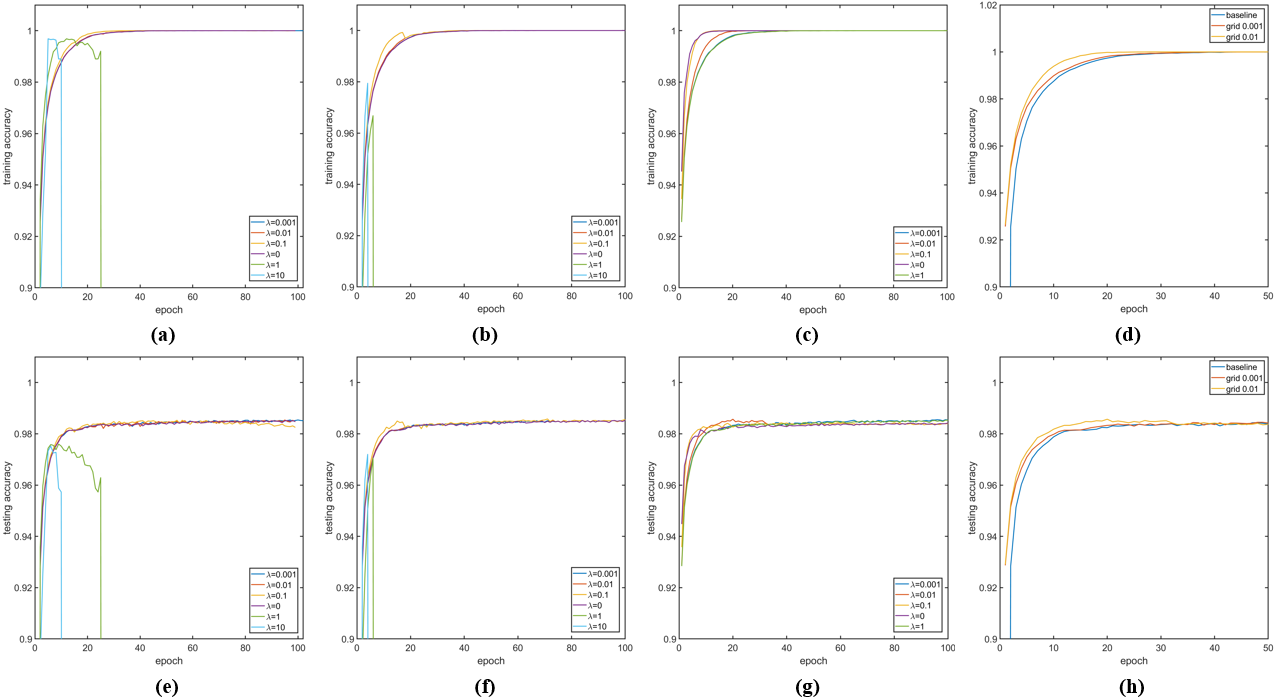
\includegraphics[width=1\textwidth]{Figs/accuracy.png}
\caption{The accuracy curves with various multipliers $\lambda \in \{0.001, 0.01, 0.1, 0, 1, 10\}$, where the x- and y-axes denote the epoch and accuracy, respectively. Training accuracy curves provided (a) Baseline $\Theta_0$, (b) Baseline $\Theta_{t'}$, and (c) Grid Search. Testing accuracy curves provided (e) Baseline $\Theta_0$, (f) Baseline $\Theta_{t'}$, and (g) Grid Search. Comparison (d) training and (h) testing accuracy curves between Baseline $\Theta_0$, Grid 0.001, and Grid 0.01. }
\label{fig:accuracy}
\end{figure*}
\section{Experiments}  \label{sec:experiments}
In this section, we conduct several experiments to evaluate the effectiveness of the proposed UNK kernel. 

\subsection{Datasets and Configurations}
Following the experimental configurations of Lee et al.~\citep{lee2018:NNGP}, we conduct the empirical evaluations on a two-hidden-layer MLP trained with various $\lambda$. The conducted dataset is the \href{http://yann.lecun.com/exdb/mnist/}{MNIST handwritten digit} data, which comprises a training set of 60,000 examples and a testing set of 10,000 examples in 10 classes, where each example is centered in a $28 \times 28$ image. 

For the classification tasks, the class labels are encoded into an opposite regression formation, where the correct label is marked as 0.9 and the incorrect one is marked as 0.1~\citep{zhang2022:NNGP}. Here, we employ 5000 hidden neurons and the \textit{softmax} activation function. Similar to~\citep{arora2019:NNGP}, all weights are initialized with a Gaussian distribution of the mean 0 and variance $0.3/n_l$ for $l \in [L]$. We also force the batch size and the learning rate as 64 and 0.001, respectively. All experiments were conducted on Intel Core-i7-6500U.



\subsection{Experiments for Effects of Various Multipliers $\lambda$}  \label{subsec:experiment_lamda}
The experiments aim to leverage the effects of various $\lambda$ on the performance of the UNK kernel. According to the recursive formulation of $K_{\textrm{UNK}}^{(l)}$, it is evident that $\lambda$ balances the gradient and regularizer. From the perspective of theoretical effects, the absolute value of $\lambda$ indicates not only the limiting convergence rate of $K_{\textrm{UNK}}^{(l)}$ but also the optimal solution of Eq.~\eqref{eq:min}. Provided $\Theta_{t'}$, we can compute the optimal solution $\lambda^*_{t}$ at current epoch stamp $t$ as follows
\begin{equation}  \label{eq:optimal}
    \lambda^*_t = \arg\min_{t'} ~ \hbar(\Theta_{t+\dif t}) - \hbar(\Theta_t) \ ,
\end{equation}
where $\Theta_{t+ \dif t} = \Theta_t  - {\dif \hbar(\Theta_t)}/{\dif \Theta_t} - \lambda_{t'} \Theta_{t'}$. This optimization problem can be solved by some mature algorithms, such as Bayesian optimization or grid search. Here, we conjecture that $\lambda^*_t$ is an effective indicator for identifying the optimal trajectory of the UNK kernel.

Here, we set the investigated values of the multiplier $\lambda$ to $\{0.001, 0.01, 0.1, 0, 1, 10\}$ and employ three types of studied models as follows
\[
\left\{\begin{aligned}
\textrm{Baseline $\Theta_0$}:&\quad  \frac{\dif \Theta}{\dif t} =  -  \frac{\dif \hbar(\Theta_t)}{\dif \Theta_t} - \lambda \Theta_0 \ ,   \\
\textrm{Baseline $\Theta_{t'}$}:&\quad  \frac{\dif \Theta}{\dif t} =  -  \frac{\dif \hbar(\Theta_t)}{\dif \Theta_t} - \lambda_{t'} \Theta_{t'} \ ,   \\
\textrm{Grid Search}:&\quad  \frac{\dif \Theta}{\dif t} =  -  \frac{\dif \hbar(\Theta_t)}{\dif \Theta_t} - \lambda^*_t \Theta_{t-\dif t} \ ,
\end{aligned}\right.
\]
where the optimization problem in Eq.~\eqref{eq:optimal} is solved by gird search with the granularity of 0.001 and 0.01, which are denoted as Grid 0.001 and Grid 0.01, respectively. 

Figure~\ref{fig:accuracy} draws various multipliers and the corresponding accuracy curves. There are several observations that (1) the performance of the training algorithms led by Eq.~\eqref{eq:min} is comparable to those of typical gradient descent in various configurations, (2) $\lambda=1$ and $\lambda=10$ are too large to hamper the performance of the UNK kernel, and (3) Grid 0.01 provides a starting point for higher accuracy and achieves the fastest convergence speed and best accuracy. The above observations not only show the effectiveness of our proposed UNK kernel, but also coincide with our theoretical conclusions that the UNK kernel converges to the NNGP kernel as $t \to \infty$ and a smaller value of $\lambda$ may lead to a larger convergence rate.

In detail, Table~\ref{tab:accuracy_training} lists the optimal trajectory and the corresponding training accuracy of Grid 0.001 and Grid 0.01 over the epoch. It is observed that (1) the optimal trajectory of the UNK kernel and the path of typical gradient descent are not completely consistent, and (2) both Grid 0.001 and Grid 0.01 achieve faster convergence speed and better accuracy than those of the baseline methods. These results further demonstrate the effectiveness of our proposed UNK kernel. 


\begin{table}[!htb]
\centering
\begin{tabular}{l|l|ll|ll}
    \toprule
        Epoch & Baseline & Grid 0.001 & ~ & Grid 0.01 & ~ \\ \hline
        $t$ & ACC. & $\lambda^*_t$ & ACC. & $\lambda^*_t$ & ACC. \\
        \hline
        1  & 0.1289  & 0.0100  & 0.9257  & 0.0800  & 0.9266  \\ 
        2  & 0.9256  & 0.0020  & 0.9506  & 0.0800  & 0.9521  \\ 
        3  & 0.9504  & 0.0040  & 0.9631  & 0.0900  & 0.9656  \\ 
        4  & 0.9629  & 0.0080  & 0.9708  & 0.0700  & 0.9737  \\ 
        5  & 0.9705  & 0.0070  & 0.9766  & 0.0900  & 0.9793  \\ 
        6  & 0.9763  & 0.0050  & 0.9802  & 0.1000  & 0.9839  \\ 
        7  & 0.9800  & 0.0060  & 0.9834  & 0.1000  & 0.9870  \\ 
        8  & 0.9831  & 0.0000  & 0.9858  & 0.0800  & 0.9899  \\ 
        9  & 0.9855  & 0.0080  & 0.9879  & 0.0500  & 0.9922  \\ 
        10  & 0.9875  & 0.0000  & 0.9898  & 0.0900  & 0.9939  \\ 
        11  & 0.9896  & 0.0000  & 0.9913  & 0.0600  & 0.9952  \\ 
        12  & 0.9910  & 0.0000  & 0.9923  & 0.0600  & 0.9963  \\ 
        13  & 0.9922  & 0.0040  & 0.9933  & 0.0700  & 0.9971  \\ 
        14  & 0.9931  & 0.0020  & 0.9943  & 0.0800  & 0.9977  \\ 
        15  & 0.9941  & 0.0020  & 0.9952  & 0.0500  & 0.9984  \\ 
        16  & 0.9949  & 0.0080  & 0.9959  & 0.0700  & 0.9987  \\ 
        17  & 0.9957  & 0.0060  & 0.9966  & 0.0900  & 0.9992  \\ 
        18  & 0.9963  & 0.0070  & 0.9972  & 0.0700  & 0.9995  \\ 
        19  & 0.9969  & 0.0070  & 0.9977  & 0.0000  & 0.9996  \\ 
        20  & 0.9974  & 0.0100  & 0.9981  & 0.0800  & 0.9998  \\ 
        21  & 0.9978  & 0.0070  & 0.9984  & 0.0100  & 0.9997  \\ 
        22  & 0.9982  & 0.0100  & 0.9986  & 0.0200  & 0.9999  \\ 
        23  & 0.9984  & 0.0050  & 0.9987  & 0.0000  & 0.9999  \\ 
        24  & 0.9986  & 0.0000  & 0.9989  & 0.0000  & 0.9999  \\ 
        25  & 0.9988  & 0.0050  & 0.9990  & 0.0000  & 0.9999  \\ 
        26  & 0.9989  & 0.0030  & 0.9992  & 0.0000  & 1.0000  \\ 
        \bottomrule
\end{tabular}
\caption{Illustration of $\lambda^*_t$ and the corresponding training accuracy (ACC.) of Grid 0.001 and Grid 0.01 over epoch $t$.}
\label{tab:accuracy_training}
\end{table}


\begin{figure*}[t]
\centering
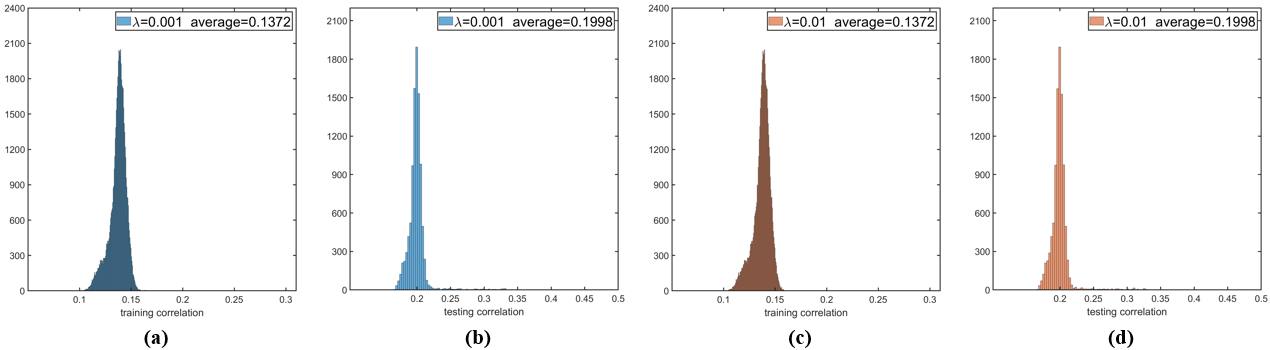
\includegraphics[width=1\textwidth]{Figs/correlation.png}
\caption{Histograms of training correlation of (a) Grid 0.001 and (c) Grid 0.01, testing correlation of (b) Grid 0.001 and (d) Grid 0.01, where x- and y-axes denote the number of instances and the corresponding correlation, respectively.}
\label{fig:correlation}
\end{figure*}
\subsection{Experiments for the UNK kernel}
This experiment investigates the representation ability of our proposed UNK kernel. The indicator is computed as
\[
\gamma^2_i = \frac{ K(T,0,\boldsymbol{x}_i) }{ K(0,0,\boldsymbol{x}_i) K(T,T,\boldsymbol{x}_i) } \ ,
\]
where $\boldsymbol{x}_i$ indicates the $i$-th instance, and $K(T,0,\boldsymbol{x}_i)$ denotes the UNK kernel trained by solving Eq.~\eqref{eq:optimal}
\[
K(t,t',\boldsymbol{x}_i) \triangleq K_{\textrm{UNK}}^{(L)} \left( t, t', \boldsymbol{s}^{L-1}_i(t), \boldsymbol{s}^{L-1}_i(t') ; \lambda^*_t\right) \ .
\]
The value of $\gamma_i$ manifests the \emph{correlation} between outputs of the UNK kernels with initialized and optimized parameters. According to the theoretical results in Section~\ref{sec:unify}, the UNK kernel is said to be \emph{valid} if the kernel outputs brought by initialized and optimized parameters are markedly discriminative. In other words, a valid UNK is able to classify digits well in this experiment, and thus $\gamma_i$ should equal $0.1 \times 1 = 0.1$, where the first 0.1 and 1 denote the accuracy of the UNK with initialized and optimized parameters, respectively. Ideally, the value of $\gamma_i$ in this experiment should trend towards 0.1, that is, $\mathbb{E}_i( \gamma_i ) = 0.1$. If $|\gamma_i|$ comes near one, the kernel cannot recognize the difference between the kernel output brought by initialized and optimized parameters, and thus the kernel is invalid.



Figure~\ref{fig:correlation} displays the (training and testing) correlation histograms and the averages for our proposed UNK kernel with the grid search granularity of 0.001 and 0.01. It is observed that the average training correlation values of Grid 0.001 and Grid 0.01 are almost 0.13 as training accuracy goes to 100\%, which implies that the trained UNK kernel is valid for classifying MNIST. This is a laudable result for the theory and development of neural kernel learning.

Notice that the average training correlation values for Grid 0.001 and Grid 0.01 are not precisely equal to 0.1, and the average testing correlation values for Grid 0.001 and Grid 0.01 are approximately 0.2 instead of the stated value of 0.1. These discrepancies could be attributed to several factors, including gaps between the softmax and labeled vectors and out-of-distribution errors. More detailed experimental results are listed in Appendix~\ref{app:experiments}.



\section{Conclusions}  \label{sec:conclusions}
In this paper, we proposed the UNK kernel, a unified framework for neural network learning that draws upon the learning dynamics associated with gradient descents and parameter initialization. Our investigation explores theoretical aspects, such as the existence, limiting properties, uniform tightness, and learning convergence of the proposed UNK kernel. Our main findings highlight that the UNK kernel exhibits behaviors akin to the NTK kernel with a finite learning step and converges to the NNGP kernel as the learning step approaches infinity. Experimental results further emphasize the effectiveness of our proposed method.


\section*{Impact Statements}
This paper presents work whose goal is to advance the field of Machine Learning. There are many potential societal consequences of our work, none of which we feel must be specifically highlighted here.



\bibliography{JMref}
\bibliographystyle{plain}
% plain, 按字母的顺序排列, 比较次序为作者-年度-标题
% unsrt, 样式同plain, 只是按照引用的先后排序
% alpha, 用作者名首字母+年份后两位作标号, 以字母顺序排序
% abbrv, 类似plain, 将月份全拼改为缩写, 更显紧凑
% ieeetr, 国际电气电子工程师协会期刊样式
% acm, 美国计算机学会期刊样式
% siam, 美国工业和应用数学学会期刊样式
% apalike, 美国心理学学会期刊样式

%%%%%%%%%%%%%%%%%%%%%%%%%%%%%%%%%%%%%%%%%%%%%%%%%%%%%%%%%%%%%%%%%%%%%%%%%%%%%%%
%%%%%%%%%%%%%%%%%%%%%%%%%%%%%%%%%%%%%%%%%%%%%%%%%%%%%%%%%%%%%%%%%%%%%%%%%%%%%%%
% APPENDIX
%%%%%%%%%%%%%%%%%%%%%%%%%%%%%%%%%%%%%%%%%%%%%%%%%%%%%%%%%%%%%%%%%%%%%%%%%%%%%%%
%%%%%%%%%%%%%%%%%%%%%%%%%%%%%%%%%%%%%%%%%%%%%%%%%%%%%%%%%%%%%%%%%%%%%%%%%%%%%%%
\newpage
\appendix
\onecolumn

{\Large\bfseries Appendix} \\~\\
This appendix provides the supplementary materials for our work ``A Unified Kernel for Neural Network Learning", constructed according to the corresponding sections therein. Before that, we first review the useful notations. Let $[N] = \{1, 2, \dots, N\}$ be an integer set for $N \in \mathbb{N}^+$, and $|\cdot|_{\#}$ denotes the number of elements in a collection, e.g., $|[N]|_{\#} = N$. Given two functions $g,h\colon \mathbb{N}^+\rightarrow \mathbb{R}$, we denote by $h=\mathbf{\Theta}(g)$ if there exist positive constants $c_1,c_2$, and $n_0$ such that $c_1g(n) \leq h(n) \leq c_2g(n)$ for every $n \geq n_0$; $h=\mathcal{O}(g)$ if there exist positive constants $c$ and $n_0$ such that $h(n) \leq cg(n)$ for every $n \geq n_0$; $h=\Omega(g)$ if there exist positive constants $c$ and $n_0$ such that $h(n) \geq cg(n)$ for every $n \geq n_0$. We define the globe $\mathcal{B}(r) = \{ \boldsymbol{x} \mid \| \boldsymbol{x} \|_2 \leq r \}$ for any $r\in\mathbb{R}^+$. Let $\mathbf{I}_n$ be the $n \times n$-dimensional identity matrix. Let $\|\cdot\|_p$ be the norm of a vector or matrix, in which we employ $p=2$ as the default. Given $\boldsymbol{x}=(x_1,\dots,x_n)$ and $\boldsymbol{y}=(y_1,\dots,y_n)$, we also define the sup-related measure as $\| \boldsymbol{x} - \boldsymbol{y} \|_{\alpha}^{\textrm{sup}} = \sup_{i\in[n]} \big| x_i - y_i \big|^{\alpha}$ for $\alpha>0$.

Let $\mathcal{C}(\mathbb{R}^{n_0};\mathbb{R}^n)$ be the space of continuous functions where $n_0,n\in\mathbb{N}$. Provided a linear and bounded functional $\mathcal{F}: \mathcal{C}(\mathbb{R}^{n_0};\mathbb{R}^n) \to \mathbb{R}$ and a function $f \in  \mathcal{C}(\mathbb{R}^{n_0};\mathbb{R}^n)$ which satisfies $f(\boldsymbol{x}) \overset{\underset{\mathrm{d}}{}}{\to} f^*$, then we have $\mathcal{F} (f(\boldsymbol{x})) \overset{\underset{\mathrm{d}}{}}{\to} \mathcal{F}(f^*)$ and $\mathbb{E} \left[ \mathcal{F} (f(\boldsymbol{x})) \right] \to \mathbb{E} \left[ \mathcal{F}(f^*) \right]$ according to General Transformation Theorem~\citep[Theorem 2.3]{van2000asymptotic} and Uniform Integrability~\citep{billingsley2013convergence}, respectively.

Throughout this paper, we use the specific symbol $K$ to denote the concerned kernel for neural network learning. The superscript $(l)$ and stamp $t$ are used for recording the indexes of hidden layers and training epochs, respectively. We denote the Gaussian distribution by $\mathcal{N}(\mu_x, \sigma_x^2)$, where $\mu_x$ and $\sigma_x^2$ indicate the mean and variance, respectively. In general, we employ $\mathbb{E}(\cdot)$ and $\mathrm{Var}(\cdot)$ to denote the expectation and variance, respectively.


\section{Theoretical Derivations of NNGP and NTK}  \label{app:two}
\subsection{NNGP and NTK}  
Here, we consider an $L$-hidden-layer fully-connected neural networks, where $n_l$ and $n_0$ indicate the number of neurons in the $l$-th hidden layer for $l \in [L]$ and input, respectively, as follows
\[
\left\{~\begin{aligned}
\boldsymbol{s}^{(0)} &= \boldsymbol{x} \ , \\
\boldsymbol{h}^{(l)} &= \mathbf{W}^{(l)} \boldsymbol{s}^{(l-1)} + \boldsymbol{b}^{(l)} \ ,\quad l \in [L] \ , \\
\boldsymbol{s}^{(l)} &= \phi( \boldsymbol{h}^{(l)} ) \ ,\quad l \in [L] \ , \\
\boldsymbol{y} &= \boldsymbol{s}^{L} \ ,
\end{aligned}\right.
\]
in which $\boldsymbol{x} \in \mathbb{R}^{n_0}$ and $\boldsymbol{y} \in \mathbb{R}^{n_L}$ indicate the variables of inputs respectively, $\boldsymbol{h}^{(l)} \in \mathbb{R}^{n_l}$ and $\boldsymbol{s}^{(l)} \in \mathbb{R}^{n_l}$ denote the pre-synaptic and post-synaptic variables of the $l$-th hidden layer respectively,  $\mathbf{W}^{(l)} \in \mathbb{R}^{n_l \times n_{l-1}} $ and $\boldsymbol{b}^{(l)} \in \mathbb{R}^{n_l} $ are the parameter variables of connection weights and bias respectively, and $\phi$ is an element-wise activation function. For convenience, we here note the parameter variables at the $t$-th epoch as $\Theta^{(l)}(t) = [ \mathbf{W}^{(l)}, \boldsymbol{b}^{(l)} ]$, and $\Theta^{(l)}(0)$ denotes the initialized parameters, of which the element obeys the Gaussian distribution $\mathcal{N}(0, \sigma^2/n_l)$.


\vspace{0.2 cm}
\noindent\textbf{Neural Network Gaussian Process (NNGP).} For any $l \in [L]$, there is a claim that the conditional variable $\boldsymbol{h}^{(l)} \mid 	\boldsymbol{s}^{(l-1)}$ obeys the Gaussian distribution. In detail, one has
\[
\begin{aligned}
	\textrm{Var} \left( \boldsymbol{h}^{(l)} \mid	\boldsymbol{s}^{(l-1)} \right) 
	&=  \textrm{Var} \left( \mathbf{W}^{(l)} \boldsymbol{s}^{(l-1)} + \boldsymbol{b}^{(l)}  \right)  \\
	&= \mathbb{E} \left(  \mathbf{W}^{(l)} \boldsymbol{s}^{(l-1)} + \boldsymbol{b}^{(l)} \right)^2 - \left[ \mathbb{E} \left( \mathbf{W}^{(l)} \boldsymbol{s}^{(l-1)} + \boldsymbol{b}^{(l)} \right) \right] ^2 \\
	&= \mathbb{E}  \left( \mathbf{W}^{(l)} \boldsymbol{s}^{(l-1)}  \right)^2 + 2  \mathbb{E}  \left( \mathbf{W}^{(l)} \boldsymbol{s}^{(l-1)} \cdot \boldsymbol{b}^{(l)} \right) + \mathbb{E}  \left( \boldsymbol{b}^{(l)} \right)^2 - \left[  \mathbb{E} \left( \mathbf{W}^{(l)} \boldsymbol{s}^{(l-1)} \right) \right]^2 \\
	&\quad - 2 \mathbb{E} \left( \mathbf{W}^{(l)} \boldsymbol{s}^{(l-1)} \right) \cdot \mathbb{E} \left( \boldsymbol{b}^{(l)} \right) - \left[  \mathbb{E} \left( \boldsymbol{b}^{(l)} \right) \right]^2 \\
	&= \mathbb{E}  \left( \mathbf{W}^{(l)} \right)^2   \mathbb{E}  \left(  \boldsymbol{s}^{(l-1)} \right)^2 + \mathbb{E}\left( \boldsymbol{b}^{(l)} \right)^2 \\
	&= \textrm{Var} \left(  \mathbf{W}^{(l)} \right) \mathbb{E} \left( \boldsymbol{s}^{(l-1)} \right)^2 + \textrm{Var} \left(  \boldsymbol{b}^{(l)} \right) \ ,
\end{aligned}
\]
where $\cdot^2$ and $\cdot$ denote the dot product, and the forth equality holds according to $\mathbb{E}  ( \mathbf{W}^{(l)} ) = \mathbf{0} \ , \quad \mathbb{E}( \boldsymbol{b}^{(l)} ) = \boldsymbol{0} $, and the elements of $\mathbf{W}^{(l)}$ and $\boldsymbol{b}^{(l)}$ are mutually independent. According to $\boldsymbol{x} \sim \mathcal{N}(\boldsymbol{0}, \mathbf{I}_{n_0})$, it is reasonable to assume that $\boldsymbol{s}^{(l-1)} \sim \mathcal{N}(\boldsymbol{0}, \mathbf{I}_{n_{l-1}} / C_{\phi})$ according to the principle of mathematical induction, where 
\[
C_{\phi} = \frac{1}{\mathbb{E}_{z \sim \mathcal{N}(0,1)} \left( \phi(z) \right)^2   }  \ .
\]
Hence, one has
\[
\boldsymbol{h}^{(l)} \mid	\boldsymbol{s}^{(l-1)}  \sim \mathcal{N} \left(  \boldsymbol{0}, \frac{\sigma^2}{n_{l-1}} \left( \frac{1}{C_{\phi}} + 1 \right) \mathbf{I}_{n_l} \right) \ .
\]
Moreover, the NNGP kernel is defined by
\[
K_{\textrm{NNGP}}^{(l)} \left( \boldsymbol{s}^{(l-1)}, \boldsymbol{s}'^{(l-1)} \right) 
= \mathbb{E} \left\langle \boldsymbol{h}^{(l)} \mid \boldsymbol{s}^{(l-1)}, \boldsymbol{h}^{(l)} \mid \boldsymbol{s}'^{(l-1)}  \right\rangle
= \sigma^2 ~\mathbb{E} \left\langle\boldsymbol{s}^{(l-1)},  \boldsymbol{s}'^{(l-1)}  \right\rangle + \sigma^2 
\]
with
\[
\lim\limits_{n_{l-1} \to \infty} \mathbb{E} \left\langle \boldsymbol{h}^{(l)} \mid \boldsymbol{s}^{(l-1)}, \boldsymbol{h}^{(l)} \mid \boldsymbol{s}^{(l-1)}  \right\rangle = \sigma^2 \left( \frac{1}{C_{\phi}} + 1 \right)  \ .
\]
In summary, we conclude the recursive form of the NNGP kernel as follows
\[
K_{\textrm{NNGP}}^{(l)} \left( \boldsymbol{s}, \boldsymbol{s}' \right) 
= \sigma^2~ \mathbb{E}_{ \boldsymbol{s} \sim \mathcal{N}(\boldsymbol{0}, K_{\textrm{NNGP}}^{(l-1)} )} \left\langle\boldsymbol{s},  \boldsymbol{s}' \right\rangle  + \sigma^2  \ .
\]


\vspace{0.2 cm}
\noindent\textbf{Neural Tangent Kernel (NTK).} The training of the concerned ANNs consists in optimizing $\boldsymbol{y} = f(\boldsymbol{x} ; \Theta)$ in the function space, supervised by a functional loss $\hbar(\Theta)$, such as the square or cross-entropy functions, where we employ $\Theta$ to denote the variable of any parameter
\[
\frac{\dif \Theta}{\dif t} = - \frac{\dif \hbar(\Theta)}{\dif \Theta} = - \frac{\dif \hbar(\Theta)}{\dif f(\boldsymbol{x} ; \Theta)} \frac{\dif f(\boldsymbol{x} ; \Theta)}{\dif \Theta} \ .
\]
The loss $\hbar(\Theta)$ is monotonically decreasing as the training epoch $t$ since
\[
\frac{\partial \hbar(\Theta)}{\partial t} = \frac{ \partial \hbar(\Theta) }{\partial \Theta} \frac{ \partial \Theta }{\partial t}  = - \nabla_{\Theta} \hbar(\Theta)  \cdot \nabla_{\Theta} \hbar(\Theta)  = - \|  \nabla_{\Theta} \hbar(\Theta) \|^2  \leq 0	\ .
\]


For any $l \geq 2$, there is a claim that the gradient variable vector $\boldsymbol{h}^{(l)} \mid \boldsymbol{s}^{(l-1)}$ obeys the Gaussian distribution. In detail, for $i,j \in \mathbb{N}^+$, one has
\[
\begin{aligned}
	\textrm{Var} \left( \frac{\partial \boldsymbol{h}^{(l)}}{\partial \mathbf{W}_{ij}^{(l-1)}} \right) 
	&= \textrm{Var} \left( \mathbf{W}^{(l)} \frac{\partial \boldsymbol{s}^{(l-1)}}{\partial \mathbf{W}_{ij}^{(l-1)}} \right)  \\
	&= \mathbb{E} \left( \mathbf{W}^{(l)} \frac{\partial \boldsymbol{s}^{(l-1)}}{\partial \mathbf{W}_{ij}^{(l-1)}} \right)^2 - \left[ \mathbb{E} \left( \mathbf{W}^{(l)} \frac{\partial \boldsymbol{s}^{(l-1)}}{\partial \mathbf{W}_{ij}^{(l-1)}} \right) \right]^2  \\
	&= \textrm{Var} \left( \mathbf{W}^{(l)} \right) \mathbb{E} \left( \frac{\partial \boldsymbol{s}^{(l-1)}}{\partial \mathbf{W}_{ij}^{(l-1)}} \right)^2 \\
	&= \textrm{Var} \left( \mathbf{W}^{(l)} \right) \mathbb{E} \left( \frac{\partial \boldsymbol{s}^{(l-1)}}{\partial \boldsymbol{h}^{(l-1)}} \right)^2 \textrm{Var} \left(  \boldsymbol{s}^{(l-2)} \right) 
\end{aligned}
\]
and 
\[
\begin{aligned}
	\textrm{Var} \left( \frac{\partial \boldsymbol{h}^{(l)}}{\partial \boldsymbol{b}_i^{(l-1)}} \right) 
	&= \textrm{Var} \left( \mathbf{W}^{(l)} \frac{\partial \boldsymbol{s}^{(l-1)}}{\partial \boldsymbol{b}_i^{(l-1)}} \right)  \\
	&= \mathbb{E} \left( \mathbf{W}^{(l)} \frac{\partial \boldsymbol{s}^{(l-1)}}{\partial \boldsymbol{b}_i^{(l-1)}} \right)^2 - \left[ \mathbb{E} \left( \mathbf{W}^{(l)} \frac{\partial \boldsymbol{s}^{(l-1)}}{\partial \boldsymbol{b}_i^{(l-1)}} \right) \right]^2 \\
	&= \textrm{Var} \left( \mathbf{W}^{(l)} \right) \mathbb{E} \left( \frac{\partial \boldsymbol{s}^{(l-1)}}{\partial \boldsymbol{b}_i^{(l-1)}} \right)^2 \\
	&= \textrm{Var} \left( \mathbf{W}^{(l)} \right) \mathbb{E} \left( \frac{\partial \boldsymbol{s}^{(l-1)}}{\partial \boldsymbol{h}^{(l-1)}} \right)^2  \ ,
\end{aligned}
\]
where ${\partial \boldsymbol{s}^{(l-1)}} / {\partial \boldsymbol{h}^{(l-1)}}$ denotes the dot operation. Hence, one has
\[
\frac{\partial \boldsymbol{h}^{(l)}}{\partial \mathbf{W}_{ij}^{(l-1)}} \sim \mathcal{N} \left(  \boldsymbol{0}, \frac{\sigma^2}{n_{l-1} C'_{\phi} C_{\phi} } \mathbf{I}_{n_{l-1}} \right) 
\quad\text{and}\quad
\frac{\partial \boldsymbol{h}^{(l)}}{\partial \boldsymbol{b}_i^{(l-1)}} \sim \mathcal{N} \left(  \boldsymbol{0}, \frac{\sigma^2}{n_{l-1} C'_{\phi} } \mathbf{I}_{n_{l-1}} \right) \ ,
\]
where 
\[
C'_{\phi} = \frac{1}{\mathbb{E}_{z \sim \mathcal{N}(0,1)} \left[ \phi'(z) \right]^2   }  \ .
\]
Moreover, the NTK kernel is defined by
\[
\begin{aligned}
K_{\textrm{NTK}}^{(l)} \left(  \boldsymbol{s}^{(l-1)}, \boldsymbol{s}'^{(l-1)} \right) 
& = K_{\textrm{NTK}}^{(l-1)} \left(  \boldsymbol{s}^{(l-2)}, \boldsymbol{s}'^{(l-2)} \right) \mathbb{E} \left\langle \frac{\partial \boldsymbol{s}^{(l-1)}}{\partial \boldsymbol{h}^{(l-1)}},  \frac{\partial \boldsymbol{s}'^{(l-1)}}{\partial \boldsymbol{h}'^{(l-1)}} \right\rangle  + K_{\textrm{NNGP}}^{(l)} \left( \boldsymbol{s}^{(l-1)}, \boldsymbol{s}'^{(l-1)} \right) \ ,
\end{aligned}
\]
for $l \geq 2$ and
\[
\begin{aligned}
	K_{\textrm{NTK}}^{(1)} \left(  \boldsymbol{x}, \boldsymbol{x}' \right)  = K_{\textrm{NNGP}}^{(1)} \left(  \boldsymbol{x}, \boldsymbol{x}' \right)  \ ,
\end{aligned}
\]

provided
\[
\lim\limits_{n_{l-1} \to \infty} \mathbb{E} \left\langle \frac{\partial \boldsymbol{h}^{(l)}}{\partial \mathbf{W}_{ij}^{(l-1)}} , \frac{\partial \boldsymbol{h}^{(l)}}{\partial \mathbf{W}_{ij}^{(l-1)}}  \right\rangle  =  \frac{\sigma^2}{C'_{\phi} C_{\phi} } 
\quad\text{and}\quad
\lim\limits_{n_{l-1} \to \infty} \mathbb{E} \left\langle \frac{\partial \boldsymbol{h}^{(l)}}{\partial \boldsymbol{b}_i^{(l-1)} } , \frac{\partial \boldsymbol{h}^{(l)}}{\partial \boldsymbol{b}_i^{(l-1)} }  \right\rangle  =  \frac{\sigma^2}{C'_{\phi} } \ .
\]




\section{Full Proof of Theorem~\ref{thm:unified} and Theorem~\ref{thm:unified_2}}  \label{app:unified}
All statistics of post-synaptic variables $\boldsymbol{s}$ can be calculated via the \emph{moment generating function}
\[
\mathcal{M}_{\boldsymbol{s}} (t) = \int \e^{t \boldsymbol{s}}  f(\boldsymbol{s}) \dif \boldsymbol{s} \ .
\]
Here, we focus on the second moment of $s= \boldsymbol{s}^{(l)}_i$ for $l \in [L]$ and $i \in [n_l]$, that is,
\[
m_2 (s,t) = \int \frac{t^2s^2}{2!}  ~f(s) \dif s = \int \frac{t^2 s^2(\Theta)}{2!}  ~f_{\Theta}(\Theta) ~\frac{\dif s(\Theta)}{\dif \Theta} \dif \Theta \ ,
\]
In the above equations, $s$ and $\Theta$ denote the variables of hidden states and parameters, respectively. Let $f_{\Theta_t}(\cdot)$ denote the probability density function of $\Theta_t$. According to the formulation of $m_2 (s)$, we should compute the probability density function $f_{\Theta}(\Theta)$. For convenience, we abbreviate $\Theta(t)$ as $\Theta_t$ throughout this proof. 


According to the introduction in Section~\ref{sec:unify}, Eq.~\eqref{eq:lamda_t'} has a general updating formulation, taking Eq.~\eqref{eq:lamda} as a special case of $t'=0$. Hence, we here take a general formula as follows
\[
\Theta_{t+ \dif t} = \Theta_t  -  \frac{\dif \hbar(\Theta_t)}{\dif \Theta_t}  - \lambda \Theta_{t'} \ ,
\]
where $\dif t$ denotes the epoch infinitesimal. Here, we omit the learning rate for simplicity. Thus, we have
\[
f_{\Theta_{t+\dif t}}( u )  = \iiint \delta(  v  ) f_{\Theta_t}(x) f_{\nabla_t}(y)  f_{\Theta_0} (z) \dif x\! \dif y\! \dif z 
\]
with
\[
\left\{~ \begin{aligned}
    f_{\Theta_t}(x) &= \frac{1}{\sigma_t \sqrt{2\pi}} \exp \left( -\frac{x^2}{2\sigma_t^2} \right)   \\
    f_{\nabla_t}(y) &= \frac{1}{\sigma_y \sqrt{2\pi}} \exp \left( -\frac{y^2}{2\sigma_y^2} \right)  \\
    f_{\Theta_0} (z) &=  \frac{1}{\sigma_z \sqrt{2\pi}} \exp \left( -\frac{z^2}{2 \sigma_z^2} \right) \\
\end{aligned}\right.
\]
where $v= u- x + y  + \lambda z $, $\nabla_t = {\dif \hbar(\Theta_t)}/{\dif \Theta_t}$, and $\delta(\cdot)$ indicates the Dirac-delta function. Besides, one has
\[
\begin{aligned}
\mathrm{Var} \left( \Theta_{t+ \dif t} \right) &~=  \textrm{Var} \left( \Theta_t  -  \nabla_t - \lambda \Theta_{t'}   \right)  \\
&~= \mathbb{E} \left( \Theta_t  -  \nabla_t - \lambda \Theta_{t'}  \right)^2 - \left[ \mathbb{E} \left( \Theta_t  -  \nabla_t - \lambda \Theta_{t'}  \right) \right] ^2 \\
&~= \textrm{Var} \left( \Theta_t  -  \nabla_t \right) + \lambda^2 \textrm{Var} \left(  \Theta_{t'}  \right)  + 2 \left[  \mathbb{E} \left( \Theta_t  -  \nabla_t \right) \mathbb{E} \left( \lambda \Theta_{t'} \right) - \mathbb{E} \left( (\Theta_t  -  \nabla_t ) \lambda \Theta_{t'}  \right)  \right] \ .
\end{aligned}
\]
Notice that $\Theta_t  -  \nabla_t$ is almost independent to $\Theta_{t'}$ as $t \to \infty$. It is observed that $\mathrm{Var} ( \Theta_{t+ \dif t} ) $ converges as $n \to \infty$ and $t \to \infty$. Thus, the variable sequence $\{ \mathrm{Var}(\Theta_t) \}_t$ is bounded. Here, we define that 
\[
\mathrm{Var} ( \Theta_{t} ) \leq \sigma_t^2 \ .
\]
Throughout this proof, we have a mild assumption of $\sigma^2 = \max_t \sigma_t^2 = \min_t \sigma_t^2$ for simplicity; Otherwise, we usually employ $\sqrt{1 - \rho_{t,t'}^2} \sigma_t \sigma_{t'}$, instead of the above assumption, where $\rho_{t,t'}$ denotes the correlation coefficient between variables of hidden states $\Theta_t$ and $\Theta_{t'}$. 

Moreover, we have
\[
f_{\Theta_{t+\dif t}}( u ) = \iiint \delta(  v  ) f_{\Theta_t}(x) f_{\nabla_t}(y)  f_{\Theta_0} (z) \dif x\! \dif y\! \dif z 
= \iint_{x,y}  f_{\Theta_t}(x) f_{\nabla_t}(y) \dif x\! \dif y  \int_{\Omega_z} f_{\Theta_0} (z) \dif z \ ,
\]
where $\Omega_z = \{ (x,y) \mid (-u+x-y)/ \lambda = 0 \}$. Thus, we can conjecture that $\Theta_{t+\dif t}$ obeys the Gaussian distribution with zero mean. Suppose that $\Theta_{t+\dif t} \sim \mathcal{N}(0, \sigma_{t+\dif t}^2) $ and
\[
f_{\Theta_{t+\dif t}}(x) = \frac{1}{\sigma_{t+\dif t} \sqrt{2\pi}} \exp \left( -\frac{x^2}{2\sigma_{t+\dif t}^2} \right) \ .
\]
Thus, we have
\[
\begin{aligned}
    m_2 (\Theta,t) &= \int \frac{t^2 s^2(\Theta)}{2!}  ~f_{\Theta}(\Theta) ~\frac{\dif s(\Theta)}{\dif \Theta} \dif \Theta \\
    &= \int \frac{t^2 s^2(\Theta)}{2!} ~\frac{1}{\sigma_{t+\dif t} \sqrt{2\pi}} \exp \left( -\frac{\Theta^2}{2\sigma_{t+\dif t}^2} \right) \frac{\dif s(\Theta)}{\dif \Theta} \dif \Theta \\
    &= \int \frac{t^2 }{2!} \phi^2(h(\Theta)) ~\frac{1}{\sigma_{t+\dif t} \sqrt{2\pi}} \exp \left( -\frac{\Theta^2}{2\sigma_{t+\dif t}^2} \right) \frac{\dif \phi(h(\Theta))}{\dif \Theta} \dif \Theta  \ ,
\end{aligned}
\]
where $h(\cdot)$ corresponds to $\boldsymbol{h}_i^{(l)}(\cdot)$. The above equation can be extended to the vectorized formulation in detail, where provided $s=\boldsymbol{s}^{(l)}$ and $h=\boldsymbol{h}^{(l)}$, one has
\[
m_2 \left( \mathbf{W}^{(l)},t \right) = \int \frac{t^2 }{2!} \phi^2 \left(\mathbf{W}^{(l)} \boldsymbol{s}^{(l-1)} + \boldsymbol{b}^{(l)} \right) ~\frac{1}{\sqrt{2\pi |\mathbf{\Sigma}_t|} } \exp \left( -\frac{ \mathbf{W}^{(l)}.^2 ~\mathbf{\Sigma}_t^{-1}}{2} \right) \frac{\dif \phi ( \boldsymbol{h}^{(l)} )}{\dif \boldsymbol{h}^{(l)} }  \boldsymbol{s}^{(l-1)}  \dif \mathbf{W}^{(l)} \ ,
\]
\[
m_2 \left( \boldsymbol{b}^{(l)},t \right) = \int \frac{t^2 }{2!} \phi^2 \left(\mathbf{W}^{(l)} \boldsymbol{s}^{(l-1)} + \boldsymbol{b}^{(l)} \right) ~\frac{1}{\sqrt{2\pi |\mathbf{\Sigma}_t|} } \exp \left( -\frac{ \boldsymbol{b}^{(l)}.^2 ~\mathbf{\Sigma}_t^{-1}}{2} \right) \frac{\dif \phi ( \boldsymbol{h}^{(l)} )}{\dif \boldsymbol{h}^{(l)} }  \boldsymbol{1}_{n_l \times 1}  \dif \boldsymbol{b}^{(l)} \ ,
\]
and
\[
m_2 \left( \Theta,t \right) = \int \frac{t^2 }{2!} \phi^2 \left( \boldsymbol{h}^{(l)} (\Theta) \right) ~\frac{1}{\sigma_t \sqrt{2\pi}} \exp \left( -\frac{\Theta^2}{2\sigma_t^2} \right) \frac{\dif \phi ( \boldsymbol{h}^{(l)}(\Theta) )}{\dif \boldsymbol{h}^{(l)}(\Theta) }  \mathbf{W}^{(l)} \frac{\dif \boldsymbol{s}^{(l-1)}(\Theta) }{\dif \Theta} \dif \Theta \ , \quad \textrm{otherwise} \ ,
\]
where $\mathbf{\Sigma}_t$ indicates the corresponding variance matrix. Furthermore, provided two stamps $t$ and $t+\dif t$, we have
\[
\begin{aligned}
    \mathbb{E} \left\langle \Theta_{t+\dif t}, \Theta_t  \right\rangle &= m_2( \Theta_{t+\dif t}, \Theta_t, t+\dif t, t ) \\
    &= \iint \frac{t (t+\dif t)}{2!} \Delta \left( \Theta_{t+\dif t}, \Theta_t, t+\dif t, t \right) f_{\Theta_{t+\dif t},\Theta_t} \left( \Theta_{t+\dif t}, \Theta_t \right) \dif \Theta_{t+\dif t} \dif \Theta_t \ ,
\end{aligned}
\]
where
\[
\Delta \left( \Theta_{t+\dif t}, \Theta_t, t+\dif t, t \right) = 
\phi \left( \boldsymbol{h}^{(l)} (\Theta_{t+\dif t}) \right) \cdot \phi \left( \boldsymbol{h}'^{(l)} (\Theta_t) \right) \cdot \frac{\dif \phi(\boldsymbol{h}^{(l)} \left( \Theta_{t+\dif t}) \right)}{\dif \Theta_{t+\dif t}} \cdot \frac{\dif \phi(\boldsymbol{h}'^{(l)} \left( \Theta_t) \right)}{\dif \Theta_t} 
\]
and
\[
f_{\Theta_{t+\dif t},\Theta_t} \left( \Theta_{t+\dif t}, \Theta_t \right) = 
\frac{1}{2\pi\sqrt{1-\rho_{t+\dif t, t}^2} } \exp \left[ \frac{-1}{2(1-\rho_{t+\dif t, t}^2)} \left( \frac{\Theta_{t+\dif t}}{\sigma_{t+\dif t}} - \rho_{t+\dif t,t}\frac{\Theta_t}{\sigma_t} \right)^2 \right] \ ,
\]
in which $\rho_{t+\dif t, t}$ denotes the correlation coefficient between $\Theta_{t+\dif t}$ and $\Theta_t$. The estimation of the second moment has been written as a general formula, which can be solved by some mature statistical methods, such as the replica calculation~\citep{mezard1987:Replica}. 

By direct calculations, we can obtain the concerned kernel
\[
K_{\textrm{UNK}}^{(l)} \left( t, t', \boldsymbol{s}^{(l-1)}, \boldsymbol{s}'^{(l-1)} \right)  = \exp\left( \frac{ (t'-t) ~|\lambda|}{\sigma^2} \right) \mathbb{E} \left\langle \frac{\partial \boldsymbol{h}^{(l)}(\Theta_t)}{\partial \Theta_t} , \frac{\partial \boldsymbol{h}'^{(l)}(\Theta_{t'})}{\partial \Theta_{t'}}  \right\rangle \ ,
\]
or
\[
K_{\textrm{UNK}}^{(l)} \left( t, t', \boldsymbol{s}^{(l-1)}, \boldsymbol{s}'^{(l-1)} \right)  = \exp\left( \frac{ (t'-t) ~|\lambda|}{\sqrt{1-\rho_{t,t'}^2}\sigma_{t}\sigma_{t'}} \right) \mathbb{E} \left\langle \frac{\partial \boldsymbol{h}^{(l)}(\Theta_t)}{\partial \Theta_t} , \frac{\partial \boldsymbol{h}'^{(l)}(\Theta_{t'})}{\partial \Theta_{t'}}  \right\rangle \ , 
\]
for $\sigma^2 \neq \sqrt{1-\rho_{t,t'}^2}\sigma_{t}\sigma_{t'}$. Here, $\boldsymbol{s}^{(l-1)}$ and $\boldsymbol{s}'^{(l-1)}$ are variables led by $\Theta_t$ and $\Theta_{t'}$, respectively. Similar to the NNGP and NTK kernels, the unified kernel is also of a recursive form as follows:
\begin{equation}  \label{eq:recursive_app}
\begin{aligned}
K_{\textrm{UNK}}^{(l)} \left( t, t', \boldsymbol{s}^{(l-1)}, \boldsymbol{s}'^{(l-1)} \right) =&~ K_{\textrm{UNK}}^{(l-1)} \left( t, t',  \boldsymbol{s}^{(l-2)}, \boldsymbol{s}'^{(l-2)} \right) \mathbb{E} \left\langle \frac{\partial \boldsymbol{s}^{(l-1)}}{\partial \boldsymbol{h}^{(l-1)}} \Big|_{\Theta_t},  \frac{\partial \boldsymbol{s}'^{(l-1)}}{\partial \boldsymbol{h}'^{(l-1)}} \Big|_{\Theta_{t'}} \right\rangle \\
&+ \exp\left( \frac{ (t'-t) ~|\lambda|}{ \sqrt{1-\rho_{t,t'}^2}\sigma_{t}\sigma_{t'} } \right) K_{\textrm{NNGP}}^{(l)} \left( \boldsymbol{s}^{(l-1)}(\Theta_t), \boldsymbol{s}'^{(l-1)}(\Theta_{t'}) \right) \ .
\end{aligned} 
\end{equation}


Next, we will analyze the limiting properties of $K_{\textrm{UNK}}^{(l)}$.
\begin{itemize}
    \item In the case of $\lambda=0$, it is obvious that 
    \[
    \exp\left( \frac{ (t'-t) ~|\lambda=0|}{\sqrt{1-\rho_{t,t'}^2}\sigma_{t}\sigma_{t'}} \right) = 1 \ ,
    \]
    and thus, Eq.~\eqref{eq:our_kernel_1} is degenerated as the NTK kernel
    \[
    K_{\textrm{UNK}}^{(l)} \left( t, t', \boldsymbol{s}^{(l-1)}, \boldsymbol{s}'^{(l-1)} ; \lambda=0 \right) = K_{\textrm{NTK}}^{(l)} \left(  \boldsymbol{s}^{(l-1)}, \boldsymbol{s}'^{(l-1)} \right)  \ .
    \]
    We provide another proof that originates from Eq.~\eqref{eq:lamda} with $\lambda=0$ in Appendix~\ref{app:lamda=0}.
    \item In the case of $\lambda \neq 0$ and $t=t'$, one has
    \[
    \exp\left( \frac{ (t-t) ~|\lambda|}{\sqrt{1-\rho_{t,t'}^2}\sigma_{t}\sigma_{t'}} \right) = 1 \ ,
    \]
    and thus, Eq.~\eqref{eq:our_kernel_1} equals the NTK kernel
    \[
    K_{\textrm{UNK}}^{(l)} \left( t, t, \boldsymbol{s}^{(l-1)}, \boldsymbol{s}'^{(l-1)} \right) = K_{\textrm{NTK}}^{(l)} \left(  \boldsymbol{s}^{(l-1)}, \boldsymbol{s}'^{(l-1)} \right) \ .
    \]
    \item In the case of $\lambda \neq 0$ and $t-t' \to \infty$, we conjecture that
    \[
    \lim\limits_{t-t' \to \infty} K_{\textrm{UNK}}^{(l)} \left( t, t', \boldsymbol{s}^{(l-1)}, \boldsymbol{s}'^{(l-1)} \right) \to K_{\textrm{NNGP}}^{(l)} \left(  \boldsymbol{s}^{(l-1)}, \boldsymbol{s}'^{(l-1)} \right) \ .
    \]
    According to Eq.~\eqref{eq:recursive_app}, one has
    \[
    \begin{aligned}
       \int_{t'}^t K_{\textrm{UNK}}^{(l)} & \left( t, t', \boldsymbol{s}^{(l-1)}, \boldsymbol{s}'^{(l-1)} \right) \dif t \\
       =&~ \int_{t'}^t K_{\textrm{UNK}}^{(l-1)} \left( t, t',  \boldsymbol{s}^{(l-2)}, \boldsymbol{s}'^{(l-2)} \right) \mathbb{E} \left\langle \frac{\partial \boldsymbol{s}^{(l-1)}}{\partial \boldsymbol{h}^{(l-1)}} \Big|_{\Theta_t},  \frac{\partial \boldsymbol{s}'^{(l-1)}}{\partial \boldsymbol{h}'^{(l-1)}} \Big|_{\Theta_{t'}} \right\rangle \dif t \\
       &+ \int_{t'}^t \exp\left( \frac{ (t'-t) ~|\lambda|}{\sqrt{1-\rho_{t,t'}^2}\sigma_{t}\sigma_{t'}} \right) K_{\textrm{NNGP}}^{(l)} \left( \boldsymbol{s}^{(l-1)}(\Theta_t), \boldsymbol{s}'^{(l-1)}(\Theta_{t'}) \right) \dif t \\
       =&~  \int_{t'}^t \left[ \frac{\sqrt{1-\rho_{t,t'}^2}\sigma_{t}\sigma_{t'}}{|\lambda|} \exp\left( \frac{ (t'-t) ~|\lambda|}{\sqrt{1-\rho_{t,t'}^2}\sigma_{t}\sigma_{t'}} \right) \right]_{\partial t} K_{\textrm{NNGP}}^{(l)} \left( \boldsymbol{s}^{(l-1)}(\Theta_t), \boldsymbol{s}'^{(l-1)}(\Theta_{t'}) \right) \dif t \\
       &+ \int_{t'}^t \exp\left( \frac{ (t'-t) ~|\lambda|}{\sqrt{1-\rho_{t,t'}^2}\sigma_{t}\sigma_{t'}} \right) \left[ \frac{\sigma^2}{|\lambda|} K_{\textrm{NNGP}}^{(l)} \left( \boldsymbol{s}^{(l-1)}(\Theta_t), \boldsymbol{s}'^{(l-1)}(\Theta_{t'}) \right) \right]_{\partial t}  \dif t \\
       =&~ \frac{\sqrt{1-\rho_{t,t'}^2}\sigma_{t}\sigma_{t'}}{|\lambda|} \int_{t'}^t \left[  \exp\left( \frac{ (t'-t) ~|\lambda|}{\sqrt{1-\rho_{t,t'}^2}\sigma_{t}\sigma_{t'}} \right) K_{\textrm{NNGP}}^{(l)} \left( \boldsymbol{s}^{(l-1)}(\Theta_t), \boldsymbol{s}'^{(l-1)}(\Theta_{t'}) \right)  \right]_{\partial t}  \dif t \ ,
    \end{aligned}
    \]
    where $[\cdot]_{\partial t}$ denotes the differential operation with respect to $t$. Thus, for any $t'$, it is easy to prove that 
    \[
    \lim\limits_{t\to\infty} \int_{t'}^t K_{\textrm{UNK}}^{(l)} \left( t, t', \boldsymbol{s}^{(l-1)}, \boldsymbol{s}'^{(l-1)} \right) \dif t = \frac{\sqrt{1-\rho_{t,t'}^2}\sigma^2}{|\lambda|} K_{\textrm{NNGP}}^{(l)} \left( \boldsymbol{s}^{(l-1)}, \boldsymbol{s}'^{(l-1)}\right) \ .
    \]
    Here, we consider that the correlation coefficient $\rho_{t,t'}$ is negatively proportional to $t-t'$ since the variable correlation becomes smaller as the stamp gap increases. Generally, we employ 
    \[
    \rho_{t,t'} = \mathbf{\Theta} \left( \frac{1}{t-t'} \right)
    \quad\textrm{and}\quad
    \lim\limits_{t-t' \to \infty} \frac{\rho_{t,t'}}{t-t'} = C \in \mathbb{R} \ .
    \]
    Thus, we can obtain 
    \[
    \lim\limits_{t-t' \to \infty} K_{\textrm{UNK}}^{(l)} \left( t, t', \boldsymbol{s}^{(l-1)}, \boldsymbol{s}'^{(l-1)} \right) = K_{\textrm{NNGP}}^{(l)} \left(  \boldsymbol{s}^{(l-1)}, \boldsymbol{s}'^{(l-1)} \right) \ ,
    \]
    in which we omit the constant multiplier.
\end{itemize}

Considering the mild assumption of $\sigma^2 = \max_t \sigma_t^2 = \min_t \sigma_t^2$, as mentioned above, we can further simplify these conclusions from
\[
\sqrt{1-\rho_{t,t'}^2}\sigma_{t}\sigma_{t'} \to \sigma^2 
\quad\textrm{as}\quad
t-t' \in \mathbb{R}^+ \ .
\]
This completes the proof. $\hfill\square$




\section{For the case of $\lambda=0$}  \label{app:lamda=0}
For the case of $\lambda=0$, we can update $\Theta$ from 
\[
\Theta_{t+ \dif t} = \Theta_t  -  \frac{\dif \hbar(\Theta)}{\dif \Theta} \Big|_t \ .
\]
Here, we omit the learning rate for simplicity. For convenience, we abbreviate $\Theta(t)$ as $\Theta_t$. It is observed that
\[
\mathrm{Var} \left( \Theta_{t+ \dif t} \right) =  \textrm{Var} \left( \Theta_t  -  \nabla_t  \right) = \mathbb{E} \left( \Theta_t  -  \nabla_t \right)^2 - \left[ \mathbb{E} \left( \Theta_t  -  \nabla_t \right) \right] ^2 \ .
\]
It is observed that $\mathrm{Var} ( \Theta_{t+ \dif t} ) $ converges as $n \to \infty$ and $t \to \infty$. Thus, the variable sequence $\{ \mathrm{Var}(\Theta_t) \}_t$ is bounded. Here, we define that 
\[
\mathrm{Var} ( \Theta_{t} ) \leq \sigma_t^2 \quad \text{and}\quad \sigma^2 = \max_t ~\sigma_t^2 \ .
\]
Let $f_{\Theta_t}(\cdot)$ denote the probability density function of $\Theta(t)$. Thus, we have
\[
f_{\Theta_{t+\dif t}}( u )  = \iint \delta(  v  ) f_{\Theta_t}(x) f_{\nabla_t}(y)  \dif x\! \dif y\!  
\]
with
\[
\left\{~ \begin{aligned}
    f_{\Theta_t}(x) &= \frac{1}{\sigma_x \sqrt{2\pi}} \exp \left( -\frac{x^2}{2\sigma_x^2} \right)   \\
    f_{\nabla_t}(y) &= \frac{1}{\sigma_y \sqrt{2\pi}} \exp \left( -\frac{y^2}{2\sigma_y^2} \right)  \\
\end{aligned}\right.
\]
where $v= u- x + y$, $\nabla_t = {\dif \hbar(\Theta_t)}/{\dif \Theta_t}$, and $\delta(\cdot)$ indicates the Dirac-delta function. Thus, it is feasible to conjecture that $\Theta_{t+\dif t}$ obeys the Gaussian distribution with zero mean. We define $\Theta_{t+\dif t} \sim \mathcal{N}(0, \sigma_u^2) $.

Thus, the second moment in $\mathcal{M}_{\boldsymbol{s}} (\cdot)$ becomes 
\[
m_2 (s) = \int s^2  ~f(s) \dif s = \int s^2(\Theta) ~\frac{1}{\sigma_u \sqrt{2\pi}} \exp \left( -\frac{s^2(\Theta)}{2\sigma_u^2} \right) \frac{\dif s(\Theta)}{\dif \Theta} \dif \Theta \ ,
\]
where $s= \boldsymbol{s}^{(l)}_i$ for $l \in [L]$ and $i \in [n_l]$. Based on the above equations, we can obtain the concerned kernel
\[
K_{\textrm{UNK}}^{(l)} \left( t, t', \boldsymbol{s}^{(l-1)}, \boldsymbol{s}'^{(l-1)} ; \lambda=0 \right) = \mathbb{E} \left\langle \frac{\partial \boldsymbol{h}^{(l)}(\Theta_t)}{\partial \Theta_t} , \frac{\partial \boldsymbol{h}'^{(l)}(\Theta_{t'})}{\partial \Theta_{t'}}  \right\rangle  \ ,
\]
which coincides with the theory of NTK and our proposed unified kernel. $\hfill\square$



\section{Uniform Tightness of $K_{\textrm{UNK}}^{(l)}$} \label{app:tightness}
Lemma~\ref{lemma:tightness} can be straightforwardly derived from Kolmogorov Continuity Theorem~\cite{stroock1997:Kolmogorov}, provided the Polish space $(\mathbb{R}, |\cdot|)$. 

\subsection{Full Proof of Lemma~\ref{lemma:tightness_1}}
It suffices to prove that 
\begin{itemize}
    \item[1)] $\boldsymbol{x}=\boldsymbol{0}$ is a tight point of $\boldsymbol{s}_t(\boldsymbol{x})$ ($t \in [T]$) in $\mathcal{C}(\mathbb{R}^{n_0},\mathbb{R})$. This conjecture is self-evident since every probability measure in $(\mathbb{R}, |\cdot|)$ is tight~\cite{zhang2021:arise}.
    \item[2)] The statistic $(\boldsymbol{s}_1(\boldsymbol{0})+ \dots + \boldsymbol{s}_t(\boldsymbol{0})) / t$ converges in distribution as $t \to \infty$. This conjecture has been proved by Theorem~\ref{thm:unified_2}.
\end{itemize}
Therefore, we finish the proof of this lemma.  $\hfill\square$


\subsection{Full Proof of Lemma~\ref{lemma:tightness_2}}
This proof follows mathematical induction. Before that, we show the following preliminary result. Let $\theta$ be one element of the augmented matrix $(\mathbf{W}^{(l)}, \boldsymbol{b}^{(l)})$ at the $l$-th layer, then we can formulate its characteristic function as
\[
\varphi(t) = \mathbb{E}\left[ \e^{\mathrm{i}\theta t} \right] = \e^{-\eta^2 t^2/2} \quad\text{with}\quad \theta \sim \mathcal{N}(0,\eta^2) \ ,
\]
where $\mathrm{i}$ denotes the imaginary unit with $\mathrm{i} = \sqrt{-1}$. Thus, the variance of hidden random variables at the $l$-th layer becomes
\begin{equation} \label{eq:sigma}
	\sigma^2_l = \eta^2 \left[ 1 + \frac{1}{n_l}  \big\| \varphi \circ \boldsymbol{s}^{(l-1)} \big\| \right] \ .
\end{equation}

Next, we provide two useful definitions from~\citep{zhang2022:NNGP}.
\begin{definition} \label{def:well_posed}
A  function $\phi:\mathbb{R}\to\mathbb{R}$ is said to be \textbf{well-posed}, if $\phi$ is first-order differentiable, and its derivative is bounded by a certain constant $C_{\phi}$. In particular, the commonly used activation functions like ReLU, tanh, and sigmoid are well-posed (see Table~\ref{tab:activation}).
\end{definition}
\begin{table}[!htb]
	\centering
	\caption{Well-posedness of the commonly-used activation functions.}
	\label{tab:activation}
	\begin{tabular}{l|l}
		\toprule
		Activations $\phi$ & Well-Posedness  \\ \midrule
		ReLU & $\|\phi'(\boldsymbol{x})\| \leq 1$ \\ \midrule
		$\tanh$     & $\|\phi'(\boldsymbol{x})\| = \| 1- \sigma^2(\boldsymbol{x}) \| \leq 1$  \\ \midrule
		sigmoid  & $\|\phi'(\boldsymbol{x})\| = \| \phi(\boldsymbol{x})(1- \phi(\boldsymbol{x})) \| \leq 0.25$  \\ \bottomrule
	\end{tabular} 
\end{table}
\begin{definition} \label{def:stable_pertinent}
A matrix $\mathbf{W}$ is said to be \textbf{stable-pertinent} for a well-posed activation function $\phi$, in short $\mathbf{W} \in SP(\phi)$, if the inequality $C_{\phi} \|\mathbf{W}\| < 1$ holds.
\end{definition}


Since the activation $\phi$ is a well-posed function and $(\mathbf{W}^{(l)},\boldsymbol{b}^{(l)}) \in SP(\phi)$, we affirm that $\phi$ is Lipschitz continuous (with Lipschitz constant $L_{\phi}$). Now, we start the mathematical induction. When $t=1$, for any $\boldsymbol{x}, \boldsymbol{x}' \in \mathbb{R}^{n_0}$, we have
\[
\mathbb{E} \left[~ \| \boldsymbol{s}_t(\boldsymbol{x}) - \boldsymbol{s}_t(\boldsymbol{x}') \|_{\alpha}^{\textrm{sup}} ~\right] \leq C_{\eta,\theta,\alpha} \| \boldsymbol{x} - \boldsymbol{x}' \|_{\alpha} \ ,
\]
where $C_{\eta,\theta,\alpha} = \eta^{\alpha}~ \mathbb{E}[ |\mathcal{N}(0,1)|^{\alpha} ] $. Per mathematical induction, for $t \geq 1$, we have
\[
\mathbb{E} \left[~ \| \boldsymbol{s}_t(\boldsymbol{x}) - \boldsymbol{s}_t(\boldsymbol{x}') \|_{\alpha}^{\textrm{sup}} ~\right] \leq C_{\eta,\theta,\alpha} \| \boldsymbol{x} - \boldsymbol{x}' \|_{\alpha} \ .
\]
Thus, one has
\begin{equation} \label{eq:induction}
\mathbb{E} \left[~ \| \boldsymbol{s}_t(\boldsymbol{x}) - \boldsymbol{s}_t(\boldsymbol{x}') \|_{\alpha}^{\textrm{sup}} ~\right] 
\leq \frac{ (C_{\phi})^{\alpha} }{n_l} ~\mathbb{E}[~ |\mathcal{N}(0,1)|^{\alpha} ~]~ \Big\| \boldsymbol{s}_{t-1}(\boldsymbol{x}) - \boldsymbol{s}_{t-1}(\boldsymbol{x}') \Big\|_{\alpha}  \ ,
\end{equation}
where
\[
\begin{aligned}
C_{\phi} &= \sigma^2_0(\boldsymbol{x}) - 2 \Sigma_{\boldsymbol{x},\boldsymbol{x}'} + \sigma^2_0(\boldsymbol{x}') \\
&=  \frac{\eta^2}{n_l}~  \Big\| \phi\circ \boldsymbol{s}_{t-1}(\boldsymbol{x}) - \phi\circ \boldsymbol{s}_{t-1}(\boldsymbol{x}') \Big\|_2  \qquad\text{(~from Eq.~\eqref{eq:sigma}~)} \\
&\leq \frac{\eta^2 L_{\phi}^2}{n_l}~ \big\| \boldsymbol{s}_{t-1}(\boldsymbol{x}) - \boldsymbol{s}_{t-1}(\boldsymbol{x}') \big\|_2 \ .
\end{aligned}
\]
Thus, Eq.~\eqref{eq:induction} becomes
\[
\mathbb{E} \left[~ \| \boldsymbol{s}_t(\boldsymbol{x}) - \boldsymbol{s}_t(\boldsymbol{x}') \|_{\alpha}^{\textrm{sup}} ~\right]
\leq C'_{\eta,\theta,\alpha} \| \boldsymbol{x} - \boldsymbol{x}' \|_{\alpha} \ ,
\]
where
\[
C_{\eta,\theta,\alpha}' = \frac{(\eta L_{\phi})^{\alpha}}{n_l} \big\| \boldsymbol{s}_{t-1}(\boldsymbol{x}) - \boldsymbol{s}_{t-1}(\boldsymbol{x}') \big\|_{\alpha}~ \mathbb{E}[~ |\mathcal{N}(0,1)|^{\alpha} ~] \ .
\]
Iterating this argument, we obtain
\[
\mathbb{E} \left[~ \| \boldsymbol{s}_t(\boldsymbol{x}) - \boldsymbol{s}_t(\boldsymbol{x}') \|_{\alpha}^{\textrm{sup}} ~\right]  \leq C_{\eta,\theta,\alpha} \| \boldsymbol{x} - \boldsymbol{x}' \|_{\alpha} \ ,
\]
where 
\[
C_{\eta,\theta,\alpha} = \eta^{\alpha (t+1)} L_{\phi}^{\alpha t} ~ \mathbb{E}[~ |\mathcal{N}(0,1)|^{\alpha} ~]^{t+1} \ .
\]
The above induction holds for any positive even $\alpha$. Let $\beta = \alpha - n_0 > 0$, then this lemma is proved as desired. $\hfill\square$
	
	
	
\section{Tight Bound for Convergence} \label{app:convergence}
We begin this proof with the following lemmas.
\begin{lemma} \label{lemma:concentration}
Let $f:\mathbb{R}^{n_0} \to \mathbb{R}$ be a Lipschitz continuous function with constant $C_{n_0}$ and $P_X$ denote the Gaussian distribution $\mathcal{N}(0,\eta^2)$, then for $\forall~ \delta>0$, there exists $c >0$, s.t.
\begin{equation} \label{eq:log}
	\mathbb{P} \left( \left| f(\boldsymbol{x})-\int f \left(\boldsymbol{x}^{\prime}\right) \dif P_{X}\left(\boldsymbol{x}^{\prime}\right) \right| > \delta \right) \leq 2 \e^\frac{-c \delta^{2}}{C_{n_0}^2} \ .
\end{equation}
\end{lemma}
Lemma~\ref{lemma:concentration} shows that the Gaussian distribution corresponding to our samples satisfies the log-Sobolev inequality, i.e., Eq.~\eqref{eq:log}, with some constants unrelated to dimension $n_0$. This result also holds for the uniform distributions on the sphere or unit hypercube~\cite{nguyen2021:eigenvalues}. 

\begin{lemma} \label{lemma:input}
Suppose that $\boldsymbol{x}_1, \dots, \boldsymbol{x}_N$ are i.i.d. sampled from $\mathcal{N}(0,\eta^2)$, then with probability $1-\delta>0$, we have 
\[
\|\boldsymbol{x}_i\|_2 = \mathbf{\Theta}(\sqrt{n_0}) \quad \text{and}\quad |\langle \boldsymbol{x}_i,\boldsymbol{x}_j \rangle|^r \leq n_0 N^{-1/(r-0.5)} \ , 
\]
for $i \neq j$, where
\[
\delta \leq N \e^{-\Omega(n_0)} + N^{2} \e^{-\Omega\left(n_0 N^{-2 /(r-0.5)}\right)} \ .
\]
\end{lemma}
From Definition 1 of the manuscript, we have
\[
\int\|\boldsymbol{x}\|_{2}^{2} \dif P_X(\boldsymbol{x}) = \mathbf{\Theta}(n_0) \ .
\]
Since $\boldsymbol{x}_1, \dots, \boldsymbol{x}_n$ are i.i.d. sampled from $P_X = \mathcal{N}(0,\eta^2)$, for $\forall$ $i\in[N]$, we have $\|\boldsymbol{x}_i\|_2^2 = \mathbf{\Theta}(n_0)$ with probability at least $1- N\e^{\Omega(n_0)}$. Provided $\boldsymbol{x}_i$, the single-sided inner product $\langle \boldsymbol{x}_i,\cdot \rangle$ is Lipschitz continuous with the constant $C_{n_0} = \mathcal{O}(\sqrt{n_0})$. As such, from Lemma~\ref{lemma:concentration}, for $\forall~ j\neq i$, we have
\[
\mathbb{P} \left( |\langle \boldsymbol{x}_i,\boldsymbol{x}_j \rangle| > \delta^* \right) \leq 2 \e^{-\delta^2/C_{n_0}^2} \ .
\]
Then, for $r \geq 2$, we have
\[
\mathbb{P} \left( \max_{j\neq i} |\langle \boldsymbol{x}_i,\boldsymbol{x}_j \rangle|^r > \delta^* \right) \leq N^{2} \e^{-\Omega\left( {\delta^*}^2\right)} .
\]
We complete the proof by setting $\delta^* \leq n_0N^{-1/(r-0.5)}$. 
$\hfill\square$



\subsection{Full proof of Theorem~\ref{thm:smallest}}
We start this proof with some notations. For convenience, we force $n =|\boldsymbol{s}^{(1)}|_{\#} = |\boldsymbol{s}^{(2)}|_{\#} = \dots = |\boldsymbol{s}^{(L)}|_{\#}$, or equally, $n=n_1=\dots=n_L$. We also abbreviate the covariance $\mathrm{Cov}(\boldsymbol{s}^{(l)},\boldsymbol{s}^{(l)})$ as $\mathbf{C}_{l}$ throughout this proof.

Unfolding the $K_{\textrm{UNK}}^{(l)}$ kernel equation that omits the epoch stamp
\begin{equation} \label{eqn:kernel} 
K_{\textrm{UNK}}^{(l)} (\boldsymbol{x}_i,\boldsymbol{x}_j) = \mathbb{E}[\langle f(\boldsymbol{x}_i; \boldsymbol{\theta}), f(\boldsymbol{x}_j; \boldsymbol{\theta})\rangle], \quad\text{for}\quad \boldsymbol{x}_i, \boldsymbol{x}_j \in \mathcal{D} \ ,   
\end{equation}
we have 
\begin{equation} \label{eq:K_cov}
K_{\textrm{UNK}}^{(l)} (\boldsymbol{x}_i, \boldsymbol{x}_j) = \frac{1}{M_{\boldsymbol{z}}} \left[ \sum_{\kappa} \varphi_{\kappa} + \sum_{\kappa_1 \neq \kappa_2} \phi_{\kappa_1,\kappa_2} \right] \ ,
\end{equation}
where
\[
\left\{\begin{aligned}
	&\varphi_l = \mathbb{E} \left[ \langle \boldsymbol{s}^{l}, \boldsymbol{s}^{(l)} \rangle \right] \ , \\
	&\psi_{l_1l_2} = \sum\nolimits_{p,q} \mathbb{E} \left[ \boldsymbol{s}_p^{(l_1)} \boldsymbol{s}_q^{(l_2)} \right], \quad\text{for}\quad l_1 \neq l_2 \ ,
\end{aligned} \right.
\]
in which the subscript $p$ indicates the $p$-th element of vector $\boldsymbol{s}^{(l)}$. From Theorem 1 of the manuscript, the sequence of random variables $\boldsymbol{s}^{(l)}$ is weakly dependent with $\beta(t) \to \infty$ as $t\to \infty$. Thus, $\psi_{l_1l_2}$ is an infinitesimal with respect to $|l_2-l_1|$ when $l_1 \neq l_2$.

\noindent Invoking the following equations
\begin{equation*} 
	\left\{~\begin{aligned}
		&\chi_{\min}(\mathbf{P}\mathbf{Q}) \geq \chi_{\min}(\mathbf{P}) \min_{i\in[m]} \mathbf{Q}(i,i)  \\
		&\chi_{\min}(\mathbf{P}+\mathbf{Q}) \geq \chi_{\min}(\mathbf{P}) + \chi_{\min}(\mathbf{Q}) 
	\end{aligned} \right.
\end{equation*}
into Eq.~\eqref{eq:K_cov}, we have
\begin{equation}  \label{eq:thm2_1}
    \chi_{\min}( K_{\textrm{UNK}}^{(l)} ) \geq \sum\nolimits_{l} \chi_{\min} \left( \mathbf{C}_{l} \right) \ ,
\end{equation}
and
\begin{equation}  \label{eq:thm2_2}
    chi_{\min} \left( \mathbf{C}_{l}\right) \geq \chi_{\min} \left( \mathbf{C}_{l} \right), \quad\text{for}\quad l \in [L] \ .
\end{equation}
Iterating Eq.~\eqref{eq:thm2_2} and then invoking it into Eq.~\eqref{eq:thm2_1}, we have
\begin{equation} \label{eq:thm2_3}
	\chi_{\min} \left( K_{\textrm{UNK}}^{(l)} \right) \geq \sum_l \chi_{\min}\left( \mathbf{C}_1 \right) \ .
\end{equation}
From the Hermite expansion~\cite{zhang2021:arise} of ReLU function, we have
\begin{equation} \label{eq:relu}
	\mu_{r}(\psi) = (-1)^{\frac{r-2}{2}} (r-3)!! / \sqrt{2 \pi r!} \ ,
\end{equation}
where $r \geq 2$ indicates the expansion order. Thus, we have
\begin{equation} \label{eq:thm2_4}
	\begin{aligned}
		\chi_{\min}\left( \mathbf{C}_1 \right) &= \chi_{\min}\left( \psi(\mathbf{W}^{(1)}\mathbf{X}) \psi(\mathbf{W}^{(1)}\mathbf{X})^{\top} \right) \\
		&\geq \mu_{r}(\phi)^2 \chi_{\min}\left( \mathbf{X}^{(r)} \left( \mathbf{X}^{(r)} \right)^{\top} \right) \\
		&\geq \mu_{r}(\psi)^2 \left( \min_{i\in[N]} \|\boldsymbol{x}_i\|_2^{2r} - (N-1) \max_{j\neq i} |\langle \boldsymbol{x}_i,\boldsymbol{x}_j \rangle|^r \right) \\
		&\geq \mu_{r}(\psi)^2 ~\Omega(n_0) \ ,
	\end{aligned}
\end{equation}
where the superscript $(r)$ denotes the $r$-th Khatri Rao power of the matrix $\mathbf{X}=[\boldsymbol{x}_1, \dots,\boldsymbol{x}_N]$, the first inequality follows from Eq.~\eqref{eq:relu}, the second one holds from Gershgorin Circle Theorem~\cite{salas1999gershgorin}, and the third one follows from Lemma~\ref{lemma:input}. Therefore, we can obtain the lower bound of the smallest eigenvalue by plugging Eq.~\eqref{eq:thm2_4} into Eq.~\eqref{eq:thm2_3}.

On the other hand, it is observed from Lemma~\ref{lemma:tightness} that for $l \in [L]$,
\begin{equation} \label{eq:thm2_5}
\left\{~\begin{aligned}
& \| \boldsymbol{s}_p^{(l)} \|^2_2 = \mathbb{E}_{\mathbf{W}^{(l)}_p} \left[ \psi(\mathbf{W}^{(l)}_p\boldsymbol{s}^{(l-1)})^2 \right] = \| \boldsymbol{s}_q^{(l)} \|^2, \quad\text{for}\quad \forall q \neq p ,\\
&\| \boldsymbol{s}^{(l)} \|_2^2 = \mathbb{E}_{\mathbf{W}^{(l)}} \left[ \psi(\mathbf{W}^{(l)}\boldsymbol{s}^{(l-1)})^2 \right] \leq \| \boldsymbol{s}^{(l)} \|_2^2 \ . 
\end{aligned}\right.
\end{equation}
Thus, we have
\[
\begin{aligned}
	\chi_{\min}( K_{\textrm{UNK}}^{(l)} ) &\leq \frac{\tr( K_{\textrm{UNK}}^{(l)} )}{N} = \frac{1}{N} \sum_{i}^{N} K_{\textrm{UNK}}^{(l)}(\boldsymbol{x}_i, \boldsymbol{x}_i) \\
	& \leq  \frac{1}{N} \sum_{i}^{N} \frac{1}{M_{\boldsymbol{z}}} \left[ \sum_{l} \varphi_{l} + \sum_{l_1 \neq l_2} \psi_{l_1l_2} \right] \\
	&\leq \frac{1}{N} \sum_{i}^{N}\left( \frac{1}{l} \sum_{l} \max_{j\in[N]} \|\boldsymbol{x}_j\|_2^2 + \Omega(n_0) \right) \\
	&\leq \mathbf{\Theta}(n_0) \ ,
\end{aligned}
\]
where the second inequality follows from Eq.~\eqref{eq:K_cov}, the third one follows from Eq.~\eqref{eq:thm2_5}, and the fourth one holds from Lemma~\ref{lemma:input}. This completes the proof. $\hfill\square$


\section{Supplementary Experimental Results}  \label{app:experiments}
This section provides the detailed experimental results.
Table~\ref{tab:accuracy_app} lists the optimal trajectory and the corresponding testing accuracy of Grid 0.001 and Grid 0.01 over the epoch. Figure~\ref{fig:correlation_training} draws the training correlation histograms and the averages for our proposed UNK kernel with the grid search granularity of $\{0.001, 0.01, 0.1, 0, 1, 10\}$. Figure~\ref{fig:correlation_testing} draws the testing correlation histograms and the averages for our proposed UNK kernel with the grid search granularity of $\{0.001, 0.01, 0.1, 0, 1, 10\}$. 


\begin{table*}[!htb]
    \centering
    \resizebox{1\textwidth}{!}{
    \begin{tabular}{l|ll|lll|lll}
    \toprule
        Epoch & Baseline & ~ & Grid 0.001 & ~ & ~ & Grid 0.01 & ~ & ~ \\ \hline
        $t$ & Testing ACC. & Training ACC. & $\lambda^*_t$ & Testing ACC. & Training ACC. & $\lambda^*_t$ & Testing ACC. & Training ACC. \\ \hline
        1  & 0.1325  & 0.1289  & 0.0100  & 0.9287  & 0.9257  & 0.0800  & 0.9291  & 0.9266  \\ \hline
        2  & 0.9284  & 0.9256  & 0.0020  & 0.9515  & 0.9506  & 0.0800  & 0.9527  & 0.9521  \\ \hline
        3  & 0.9514  & 0.9504  & 0.0040  & 0.9607  & 0.9631  & 0.0900  & 0.9631  & 0.9656  \\ \hline
        4  & 0.9603  & 0.9629  & 0.0080  & 0.9665  & 0.9708  & 0.0700  & 0.9693  & 0.9737  \\ \hline
        5  & 0.9658  & 0.9705  & 0.0070  & 0.9709  & 0.9766  & 0.0900  & 0.9729  & 0.9793  \\ \hline
        6  & 0.9705  & 0.9763  & 0.0050  & 0.9738  & 0.9802  & 0.1000  & 0.9757  & 0.9839  \\ \hline
        7  & 0.9733  & 0.9800  & 0.0060  & 0.9756  & 0.9834  & 0.1000  & 0.9785  & 0.9870  \\ \hline
        8  & 0.9753  & 0.9831  & 0.0000  & 0.9772  & 0.9858  & 0.0800  & 0.9795  & 0.9899  \\ \hline
        9  & 0.9769  & 0.9855  & 0.0080  & 0.9789  & 0.9879  & 0.0500  & 0.9805  & 0.9922  \\ \hline
        10  & 0.9788  & 0.9875  & 0.0000  & 0.9798  & 0.9898  & 0.0900  & 0.9818  & 0.9939  \\ \hline
        11  & 0.9800  & 0.9896  & 0.0000  & 0.9809  & 0.9913  & 0.0600  & 0.9826  & 0.9952  \\ \hline
        12  & 0.9809  & 0.9910  & 0.0000  & 0.9814  & 0.9923  & 0.0600  & 0.9833  & 0.9963  \\ \hline
        13  & 0.9813  & 0.9922  & 0.0040  & 0.9814  & 0.9933  & 0.0700  & 0.9833  & 0.9971  \\ \hline
        14  & 0.9814  & 0.9931  & 0.0020  & 0.9815  & 0.9943  & 0.0800  & 0.9837  & 0.9977  \\ \hline
        15  & 0.9815  & 0.9941  & 0.0020  & 0.9815  & 0.9952  & 0.0500  & 0.9841  & 0.9984  \\ \hline
        16  & 0.9814  & 0.9949  & 0.0080  & 0.9819  & 0.9959  & 0.0700  & 0.9848  & 0.9987  \\ \hline
        17  & 0.9816  & 0.9957  & 0.0060  & 0.9824  & 0.9966  & 0.0900  & 0.9847  & 0.9992  \\ \hline
        18  & 0.9818  & 0.9963  & 0.0070  & 0.9827  & 0.9972  & 0.0700  & 0.9851  & 0.9995  \\ \hline
        19  & 0.9825  & 0.9969  & 0.0070  & 0.9830  & 0.9977  & 0.0000  & 0.9850  & 0.9996  \\ \hline
        20  & 0.9824  & 0.9974  & 0.0100  & 0.9833  & 0.9981  & 0.0800  & 0.9857  & 0.9998  \\ \hline
        21  & 0.9831  & 0.9978  & 0.0070  & 0.9834  & 0.9984  & 0.0100  & 0.9847  & 0.9997  \\ \hline
        22  & 0.9830  & 0.9982  & 0.0100  & 0.9838  & 0.9986  & 0.0200  & 0.9850  & 0.9999  \\ \hline
        23  & 0.9831  & 0.9984  & 0.0050  & 0.9835  & 0.9987  & 0.0000  & 0.9847  & 0.9999  \\ \hline
        24  & 0.9834  & 0.9986  & 0.0000  & 0.9836  & 0.9989  & 0.0000  & 0.9843  & 0.9999  \\ \hline
        25  & 0.9835  & 0.9988  & 0.0050  & 0.9830  & 0.9990  & 0.0000  & 0.9848  & 0.9999  \\ \hline
        26  & 0.9837  & 0.9989  & 0.0030  & 0.9838  & 0.9992  & 0.0000  & 0.9845  & 1.0000  \\ \hline
        27  & 0.9834  & 0.9990  & 0.0000  & 0.9834  & 0.9992  & 0.0000  & 0.9852  & 1.0000  \\ \hline
        28  & 0.9833  & 0.9991  & 0.0000  & 0.9839  & 0.9994  & 0.0000  & 0.9848  & 1.0000  \\ \hline
        29  & 0.9834  & 0.9993  & 0.0000  & 0.9834  & 0.9994  & 0.0000  & 0.9848  & 1.0000  \\ \hline
        30  & 0.9836  & 0.9993  & 0.0020  & 0.9838  & 0.9995  & 0.0000  & 0.9850  & 1.0000  \\
        \bottomrule
    \end{tabular}  }
    \caption{Illustration of $\lambda^*_t$ and the corresponding (both training and testing) accuracy (ACC.) of Grid 0.001 and Grid 0.01 over epoch $t$.}
    \label{tab:accuracy_app}
\end{table*}


\begin{figure*}[t]
\centering
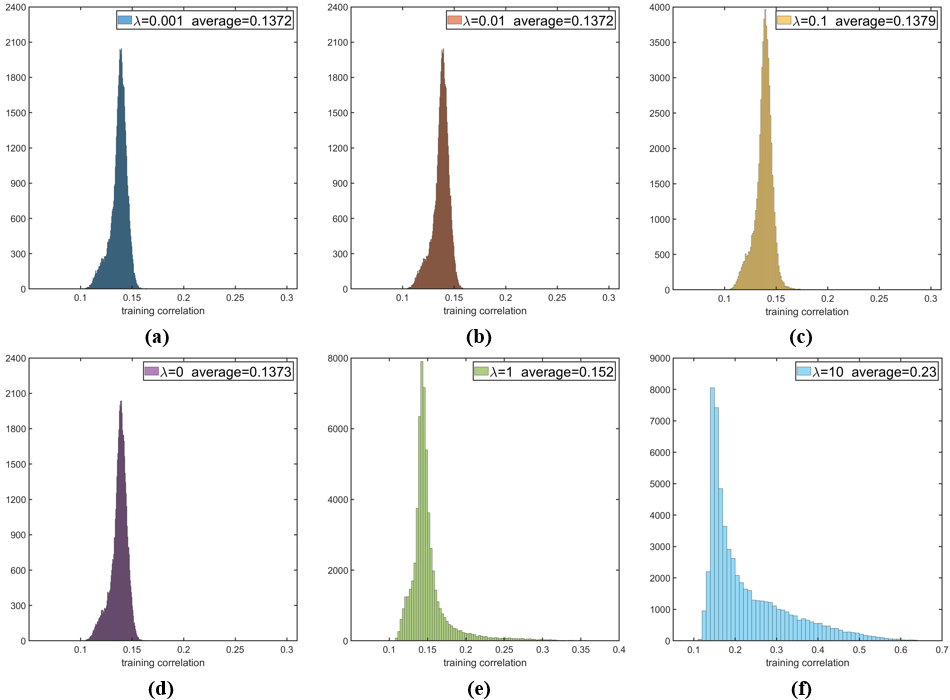
\includegraphics[width=1\textwidth]{Figs/correlation_training.png}
\caption{Histograms of training correlation of (a) Grid 0.001, (b) Grid 0.01, (c) Grid 0.1, (d) Grid 0, (e) Grid 1, and (f) Grid 10, where x- and y-axes denote the number of training instances and the corresponding correlation, respectively.}
\label{fig:correlation_training}
\end{figure*}


\begin{figure*}[t]
\centering
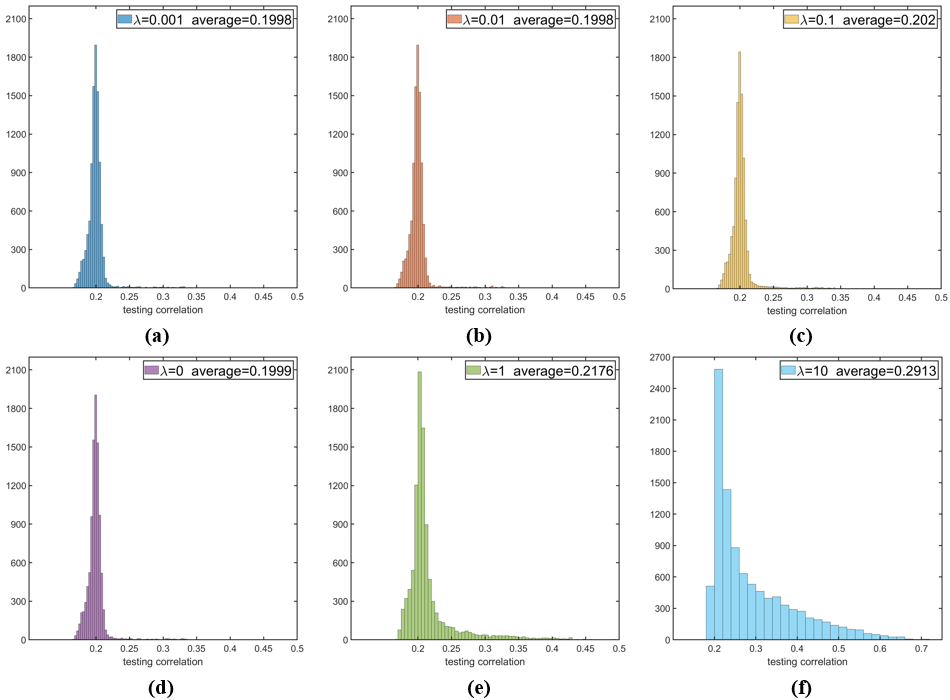
\includegraphics[width=1\textwidth]{Figs/correlation_testing.png}
\caption{Histograms of testing correlation of (a) Grid 0.001, (b) Grid 0.01, (c) Grid 0.1, (d) Grid 0, (e) Grid 1, and (f) Grid 10, where x- and y-axes denote the number of testing instances and the corresponding correlation, respectively.}
\label{fig:correlation_testing}
\end{figure*}




\end{document}
